\introparte{Esta parte recorre el desarrollo de PymeKit siguiendo las etapas del
proceso de ingeniería: requisitos, análisis, diseño, construcción, pruebas y
despliegue. De cada etapa se presentan los modelos, las decisiones y los
fragmentos de código más significativos; el resto del material ---registro de
decisiones, bitácora de incidencias, matriz de trazabilidad y código
completo--- se encuentra en el repositorio del proyecto.}

\chapter{Requisitos del Sistema}
% =====================================================================
% Capítulo: Requisitos del Sistema
% Fuentes: propuesta del TFG (Objetivo, Descripción y Alcance),
% docs/tfg/REQUISITOS.md, DECISIONES.md (ADR-004, 005, 011, 017, 020, 021)
% y borradores/04-analisis.tex. Estado de las fuentes: F3c cerrada.
% =====================================================================

En este capítulo se presentan los objetivos de negocio y del sistema, los
actores que interactúan con PymeKit y el catálogo de requisitos funcionales,
no funcionales y de información. Al final se relaciona cada requisito con el
apartado de la propuesta del TFG del que procede y con el módulo de PymeKit
que lo implementa.

Los identificadores (OBN, OBS, RF, RNF, RI) son estables: se citan en el
código mediante etiquetas \texttt{[TFG]}, en la matriz de trazabilidad del
repositorio y en esta memoria, y no se renumeran. Si un requisito cambia, se
modifica su redacción y se registra la decisión que lo justifica.

% ---------------------------------------------------------------------
\section{Objetivos de negocio}
\label{sec:req-objetivos-negocio}

Quien desarrolla un producto SaaS para pymes debe resolver, antes de escribir
su lógica de negocio, un conjunto de problemas que se repiten en casi todos
los productos de este tipo: identidad, aislamiento entre clientes, equipos y
permisos, cobro, administración interna y calidad transversal. Estos
componentes no aportan valor diferencial, pero consumen gran parte del
esfuerzo y concentran el riesgo de seguridad. De ahí se derivan los objetivos
de negocio de la tabla~\ref{tab:req-obn}.

\begin{table}[htbp]
  \centering
  \footnotesize
  \caption{Objetivos de negocio.}
  \label{tab:req-obn}
  \begin{tabularx}{\textwidth}{@{}lX@{}}
    \toprule
    \textbf{ID} & \textbf{Objetivo} \\
    \midrule
    OBN-01 & Reducir el tiempo de puesta en marcha de un nuevo producto SaaS para pymes, partiendo de una base que ya resuelve los componentes comunes. \\
    OBN-02 & Estandarizar buenas prácticas de seguridad, control de acceso y persistencia, de modo que cada producto nuevo las herede sin reimplementarlas. \\
    OBN-03 & Permitir que una pyme administre su web pública, su contenido y sus datos desde una consola, sin acceder directamente a la base de datos ni depender de un desarrollador para cada cambio. \\
    OBN-04 & Facilitar la monetización mediante suscripciones con una pasarela de pago estándar. \\
    OBN-05 & Servir como material didáctico y técnico documentado para quien reutilice la plataforma (código comentado en español, decisiones registradas y manuales). \\
    \bottomrule
  \end{tabularx}
\end{table}

Durante el desarrollo se precisó el enfoque del producto (ADR-020): PymeKit es
la base de la web de \emph{una} pyme, con una página pública, un blog
gestionado desde la consola y un inicio de sesión que puede corresponder a un
super-administrador, a personal interno o a un cliente. Los módulos SaaS
(equipos, invitaciones y suscripciones) se conservan como opcionales, porque
permiten tanto ese escenario como el de un SaaS multi-cliente.

% ---------------------------------------------------------------------
\section{Objetivos del sistema}
\label{sec:req-objetivos-sistema}

Los objetivos del sistema concretan los componentes que enumera el objetivo de
la propuesta (tabla~\ref{tab:req-obs}).

\begin{table}[htbp]
  \centering
  \footnotesize
  \caption{Objetivos del sistema y objetivos de negocio a los que contribuyen.}
  \label{tab:req-obs}
  \begin{tabularx}{\textwidth}{@{}lXl@{}}
    \toprule
    \textbf{ID} & \textbf{Objetivo del sistema} & \textbf{OBN} \\
    \midrule
    OBS-01 & Ofrecer un \textit{frontend} web con página pública, precios, blog y área privada. & 01, 03 \\
    OBS-02 & Ofrecer un \textit{backend} con API tipada y validada para la lógica de negocio y el acceso a datos. & 01 \\
    OBS-03 & Autenticar a los usuarios y autorizar cada acceso, con segundo factor y aislamiento entre cuentas aplicado en la base de datos. & 02 \\
    OBS-04 & Gestionar usuarios, cuentas de equipo, invitaciones, roles y permisos. & 01, 02 \\
    OBS-05 & Integrar una pasarela de pago para suscripciones. & 04 \\
    OBS-06 & Proporcionar una consola de administración con un CMS de datos y contenidos, con permisos y auditoría propios. & 03 \\
    OBS-07 & Ser reutilizable por configuración y estar documentado y verificado de forma automática. & 01, 05 \\
    \bottomrule
  \end{tabularx}
\end{table}

% ---------------------------------------------------------------------
\section{Actores}
\label{sec:req-actores}

\begin{description}[style=nextline]
  \item[Visitante.] Persona no identificada que consulta la web pública
        (inicio, precios y blog) y puede registrarse.
  \item[Usuario.] Persona registrada. Dispone de una cuenta personal y puede
        pertenecer a una o varias cuentas de equipo.
  \item[Propietario del equipo.] Usuario con el rol de mayor nivel en una
        cuenta de equipo; gestiona sus miembros y su suscripción.
  \item[Miembro.] Usuario de un equipo con un rol de menor nivel y, por
        tanto, con permisos limitados.
  \item[Super-administrador.] Personal del proveedor con control total de la
        plataforma y, por extensión, del CMS (ADR-014). Debe usar siempre
        segundo factor.
  \item[Personal del CMS.] Personal de la pyme o del proveedor (gestor de
        contenidos, soporte) que accede a la consola con los permisos
        limitados que le asigna el control de acceso propio del CMS
        (ADR-014, ADR-016).
  \item[Desarrollador.] Quien reutiliza PymeKit para construir un producto
        nuevo; interactúa con el repositorio, la configuración y los
        manuales, no con la interfaz.
  \item[Pasarela de pago.] Sistema externo (Stripe) que procesa los cobros y
        notifica los cambios de suscripción mediante \textit{webhooks}
        (peticiones HTTP que el sistema externo envía a la aplicación cuando
        ocurre un evento).
\end{description}

% ---------------------------------------------------------------------
\section{Requisitos funcionales}
\label{sec:req-rf}

La prioridad es \textbf{M} (imprescindible: forma parte del prototipo mínimo
que exige la propuesta) o \textbf{D} (deseable). La última columna indica el
objetivo del sistema que desarrolla cada requisito.

\begin{table}[htbp]
  \centering
  \footnotesize
  \caption{Requisitos funcionales.}
  \label{tab:req-rf}
  \begin{tabularx}{\textwidth}{@{}lXcl@{}}
    \toprule
    \textbf{ID} & \textbf{Requisito} & \textbf{Prior.} & \textbf{OBS} \\
    \midrule
    RF-01 & Interfaz web para el usuario final: página de inicio pública (\textit{landing}), precios, blog público y área privada con navegación. & M & 01 \\
    RF-02 & API de \textit{backend} para la lógica de negocio y el acceso a datos mediante funciones de servidor (\textit{server functions}) tipadas y validadas. & M & 02 \\
    RF-03 & Registro e inicio de sesión (contraseña y enlace mágico), recuperación de contraseña y verificación del correo electrónico. & M & 03 \\
    RF-04 & Segundo factor de autenticación (MFA) y proveedores OAuth configurables. & D & 03 \\
    RF-05 & Gestión de la cuenta personal: perfil, correo, contraseña y baja. & M & 04 \\
    RF-06 & Cuentas de equipo: crear equipos, invitar miembros, asignar roles y aplicar permisos por funcionalidad. & M & 04 \\
    RF-07 & Suscripciones con pasarela de pago: planes, pago (\textit{checkout}), portal de cliente y sincronización mediante \textit{webhooks}. & M & 05 \\
    RF-08 & Panel de super-administración: listar y gestionar usuarios y cuentas, bloquear, suplantar y restablecer. & M & 06 \\
    RF-09 & CMS de datos y contenidos integrado en la consola de administración: explorar y editar tablas, gestionar usuarios y almacenamiento, publicar el contenido del blog, con permisos propios. & M & 06 \\
    RF-10 & Registro de auditoría de las acciones realizadas desde el CMS. & D & 06 \\
    RF-11 & Paneles (\textit{dashboards}) configurables en el CMS. & D & 06 \\
    RF-12 & Notificaciones dentro de la aplicación y correos transaccionales. & D & 04 \\
    RF-13 & Interfaz en español, con la infraestructura de internacionalización preparada para añadir otros idiomas. & M & 07 \\
    \bottomrule
  \end{tabularx}
\end{table}

Dos requisitos han cambiado de redacción durante el proyecto, y ambos cambios
están registrados como decisiones:

\begin{itemize}
  \item \textbf{RF-09} se planteó al principio como un CMS en una aplicación
        separada que compartía la base de datos. Tras evaluar alternativas se
        decidió integrarlo en la consola de administración (ADR-011) y,
        después, usarlo también para gestionar el contenido del blog que
        publica la web (ADR-017), que es el caso de uso de «administración de
        contenidos» que pide la propuesta.
  \item \textbf{RF-13} pedía en origen una interfaz en español por defecto y
        en inglés. A petición del autor, la interfaz pasó a ofrecer
        \emph{solo} español, conservando claves, mensajes y configuración de
        idiomas como punto de extensión documentado (ADR-021).
\end{itemize}

RF-11 se identificó desde el principio como el primer candidato a recortar si
el plazo lo exigía; finalmente se implementó (ADR-019).

% ---------------------------------------------------------------------
\section{Requisitos no funcionales}
\label{sec:req-rnf}

Los requisitos no funcionales se clasifican según las características de
calidad de la norma ISO/IEC 25010~\cite{iso25010}. Cada uno se acompaña del
modo en que se verifica, para que sea comprobable y no una mera declaración
de intenciones.

\begin{table}[htbp]
  \centering
  \footnotesize
  \caption{Requisitos no funcionales, característica ISO/IEC 25010 y forma de verificarlos.}
  \label{tab:req-rnf}
  \begin{tabularx}{\textwidth}{@{}l>{\raggedright\arraybackslash}p{5.4cm}>{\raggedright\arraybackslash}p{2.2cm}X@{}}
    \toprule
    \textbf{ID} & \textbf{Requisito} & \textbf{ISO 25010} & \textbf{Verificación} \\
    \midrule
    RNF-01 & \textbf{Reutilización y configurabilidad}: la plataforma se adapta a un producto nuevo cambiando la configuración (ficheros \texttt{*.config.ts} y variables de entorno), sin tocar el núcleo. & Mantenibilidad (reusabilidad), flexibilidad & Evaluación de la reutilización: pasos y tiempo para arrancar un proyecto nuevo \\
    RNF-02 & \textbf{Seguridad}: la autorización se aplica en la base de datos (RLS) además de en la aplicación; secretos fuera del repositorio; validación de todas las entradas. & Seguridad & Pruebas pgTAP y revisiones adversariales de RLS y del código \\
    RNF-03 & \textbf{Aislamiento multi-tenant}: los datos de una cuenta no son accesibles desde otra. & Seguridad (confidencialidad) & Pruebas pgTAP de aislamiento \\
    RNF-04 & \textbf{Modularidad}: monorepo de paquetes desacoplados con dependencias explícitas y exportaciones separadas para cliente y servidor. & Mantenibilidad (modularidad) & Estructura del monorepo, comprobación de dependencias y de tipos \\
    RNF-05 & \textbf{Mantenibilidad}: TypeScript estricto, \textit{lint} y formato automáticos y código comentado en español didáctico. & Mantenibilidad (analizabilidad) & Integración continua y revisión de comentarios \\
    RNF-06 & \textbf{Calidad verificable}: pruebas unitarias, de base de datos y E2E de los casos de uso principales. & Mantenibilidad (capacidad de prueba) & Integración continua en verde \\
    RNF-07 & \textbf{Desplegabilidad}: despliegue reproducible con contenedores y en la nube, con manual de instalación. & Flexibilidad (instalabilidad) & Despliegue de prueba \\
    RNF-08 & \textbf{Usabilidad y accesibilidad}: interfaz adaptable, componentes accesibles, tema claro/oscuro y ayuda contextual en la consola. & Capacidad de interacción & Revisión manual y E2E \\
    RNF-09 & \textbf{Rendimiento razonable}: carga de datos en el servidor, caché de consultas y paginación en el CMS. & Eficiencia de desempeño & Revisión manual y pruebas puntuales \\
    \bottomrule
  \end{tabularx}
\end{table}
% VERIFICAR: nombres de las características según la edición de la norma que
% se cite (2011 o 2023; en 2023 «usabilidad» pasa a «capacidad de
% interacción» y «portabilidad» a «flexibilidad»).

% ---------------------------------------------------------------------
\section{Requisitos de información}
\label{sec:req-ri}

La tabla~\ref{tab:req-ri} recoge la información que el sistema debe almacenar.
Su modelo conceptual se desarrolla en el capítulo de Análisis
(sección~\ref{sec:ana-modelo-datos}).

\begin{table}[htbp]
  \centering
  \footnotesize
  \caption{Requisitos de información.}
  \label{tab:req-ri}
  \begin{tabularx}{\textwidth}{@{}l>{\raggedright\arraybackslash}p{3.1cm}Xl@{}}
    \toprule
    \textbf{ID} & \textbf{Información} & \textbf{Datos principales} & \textbf{RF} \\
    \midrule
    RI-01 & Usuarios & Identidad, correo, factores MFA, estado de bloqueo (gestionados por el servicio de autenticación) & 03--05 \\
    RI-02 & Cuentas & Cuenta personal o de equipo, nombre, identificador legible (\textit{slug}), propietario principal & 05, 06 \\
    RI-03 & Membresías y roles & Pertenencia de un usuario a una cuenta, rol con nivel jerárquico y permisos por funcionalidad & 06 \\
    RI-04 & Invitaciones & Correo invitado, rol ofrecido, testigo (\textit{token}), caducidad, quién invita & 06 \\
    RI-05 & Facturación & Cliente de la pasarela, suscripciones y sus líneas, pedidos de pago único & 07 \\
    RI-06 & Notificaciones & Destinatario, tipo, texto, enlace, leída o no & 12 \\
    RI-07 & Contenido del blog & Entradas (título, \textit{slug}, cuerpo en Markdown, estado, fecha de publicación, autor), categorías y etiquetas & 01, 09 \\
    RI-08 & Personal y permisos del CMS & Cuentas del CMS, roles con rango, grupos de permisos, permisos de datos, de sistema y de almacenamiento, con vigencia & 09 \\
    RI-09 & Metadatos del CMS & Por tabla: nombre visible, descripción, área de navegación, formato de visualización, configuración de columnas y diseño de la ficha; vistas guardadas & 09 \\
    RI-10 & Auditoría & Operación, tabla, registro, datos antes y después, gravedad, instantánea del autor & 10 \\
    RI-11 & Paneles & Panel, propietario, compartición por rol, \textit{widgets} y su posición en la cuadrícula & 11 \\
    \bottomrule
  \end{tabularx}
\end{table}

% ---------------------------------------------------------------------
\section{Trazabilidad con la propuesta}
\label{sec:req-trazabilidad}

La tabla~\ref{tab:req-traza-propuesta} relaciona los apartados de la
propuesta del TFG con los requisitos que los cubren y el capítulo de la
memoria donde se desarrollan. La relación inversa, de cada requisito con el
código y las pruebas que lo verifican, se presenta en el capítulo de Pruebas
(sección~\ref{sec:pru-resultados}).

\begin{table}[htbp]
  \centering
  \footnotesize
  \caption{Trazabilidad entre la propuesta del TFG, los requisitos y la memoria.}
  \label{tab:req-traza-propuesta}
  \begin{tabularx}{\textwidth}{@{}>{\raggedright\arraybackslash}X>{\raggedright\arraybackslash}p{3.6cm}>{\raggedright\arraybackslash}p{3.2cm}@{}}
    \toprule
    \textbf{Apartado de la propuesta} & \textbf{Requisitos} & \textbf{Capítulo} \\
    \midrule
    Objetivo: \textit{frontend}, \textit{backend}, autenticación, usuarios y roles, pagos y CMS & RF-01--RF-09 & Requisitos, Diseño \\
    Descripción: estructura desacoplada y configurable & RNF-01, RNF-04 & Diseño, Construcción \\
    Descripción: prototipo con gestión de usuarios, autenticación, persistencia, CMS y flujo de pago & RF-03, RF-05, RF-06, RF-07, RF-09 & Construcción, Pruebas \\
    Alcance 1: análisis y requisitos & Todo el catálogo & Requisitos, Análisis \\
    Alcance 2: arquitectura, autenticación, roles, pagos y CMS & RF-02--RF-04, RF-06--RF-09, RNF-02 & Diseño \\
    Alcance 3: modelo de datos y mecanismos de acceso & RI-01--RI-11, RNF-02, RNF-03 & Análisis, Diseño \\
    Alcance 4: implementación del prototipo y configuración para su reutilización & RF-01--RF-13, RNF-01, RNF-05 & Construcción \\
    Alcance 5: verificación de casos de uso, integración y evaluación de la reutilización & RNF-06, RNF-01 & Pruebas \\
    Alcance 6: memoria, documentación técnica y manuales & RNF-05, RNF-07 & Despliegue, anexos \\
    \bottomrule
  \end{tabularx}
\end{table}

% ---------------------------------------------------------------------
\section{Trazabilidad con los módulos}
\label{sec:req-gap}

La tabla~\ref{tab:req-gap} relaciona cada requisito con el módulo de PymeKit
que lo implementa y con la solución adoptada. El detalle de cada módulo se
presenta en el capítulo de Diseño, y las aportaciones del trabajo se resumen
en el capítulo de Construcción (sección~\ref{sec:imp-reutilizacion}).

\begin{table}[htbp]
  \centering
  \footnotesize
  \caption{Trazabilidad entre los requisitos y los módulos de PymeKit.}
  \label{tab:req-gap}
  \begin{tabularx}{\textwidth}{@{}l>{\raggedright\arraybackslash}p{4.6cm}X@{}}
    \toprule
    \textbf{Req.} & \textbf{Módulo} & \textbf{Solución} \\
    \midrule
    RF-01 & \texttt{apps/web} (rutas públicas y área privada) & Página de inicio, precios y blog en la base de datos con lectura pública por RLS (ADR-017); identidad propia \\
    RF-02 & \texttt{apps/web}, \path{packages/function-middleware} & \textit{Server functions} tipadas y validadas con \textit{middleware} de autenticación y de permisos \\
    RF-03, RF-04 & \path{packages/features/auth} & Contraseña, enlace mágico, MFA y OAuth configurables; comprobación de sesión viva en las rutas protegidas \\
    RF-05, RF-06 & \path{packages/features/accounts}, \texttt{team-accounts} & Cuentas personales y de equipo con roles y permisos por funcionalidad, aplicados por RLS \\
    RF-07 & \path{packages/billing/*} & Planes, \textit{checkout}, portal de cliente y \textit{webhooks}, como módulo opcional configurable \\
    RF-08 & \path{packages/features/admin} & Consola de super-administración compartida con el CMS y con MFA obligatorio \\
    RF-09 & \texttt{packages/cms/*}, rutas \texttt{/admin/cms} y \texttt{/api/cms} & CMS integrado en la consola (ADR-011), organizado por áreas de negocio con nombres en español (ADR-020) y con seguridad endurecida (ADR-015) \\
    RF-10 & \path{packages/cms/audit-logs} & Auditoría no falsificable que conserva el autor (ADR-018) \\
    RF-11 & \path{packages/cms/dashboards} & Paneles con \textit{widgets} sin dependencias nuevas (ADR-019) \\
    RF-12 & \path{packages/features/notifications}, \texttt{mailers}, \texttt{email-templates} & Notificaciones en la aplicación y correos transaccionales en español \\
    RF-13 & \texttt{packages/i18n} & Un único sistema de traducción y toda la interfaz en español (ADR-021) \\
    RNF-02, RNF-03 & \path{apps/web/supabase} (esquemas, RLS y pgTAP) & Autorización en la base de datos, revisiones adversariales y pruebas de aislamiento \\
    RNF-05 & \texttt{scripts/tfg}, integración continua & Comentarios didácticos en español y controles automáticos del repositorio \\
    \bottomrule
  \end{tabularx}
\end{table}



\chapter{Análisis del Sistema}
% =====================================================================
% Capítulo: Análisis del Sistema
% Fuentes: borradores/04-analisis.tex, docs/tfg/REQUISITOS.md,
% apps/web/supabase/schemas/*.sql, apps/e2e/tests, DECISIONES.md.
% Estado de las fuentes: F3c cerrada.
% =====================================================================

Este capítulo analiza el comportamiento esperado del sistema a partir de los
requisitos del capítulo anterior. Se presentan el modelo de casos de uso, con
la especificación de los principales, el modelo conceptual de datos y las
reglas de negocio que el sistema debe respetar.

% ---------------------------------------------------------------------
\section{Modelo de casos de uso}
\label{sec:ana-casos-uso}

Se han seleccionado ocho casos de uso principales que recorren todos los
módulos de la plataforma y que sirven de base para su validación
(tabla~\ref{tab:ana-cu} y figura~\ref{fig:ana-casos-uso}). Cada uno tiene una
o varias pruebas E2E que lo ejercitan (capítulo de Pruebas).

\begin{table}[htbp]
  \centering
  \footnotesize
  \caption{Casos de uso principales.}
  \label{tab:ana-cu}
  \begin{tabularx}{\textwidth}{@{}l>{\raggedright\arraybackslash}p{2.6cm}X>{\raggedright\arraybackslash}p{2.4cm}@{}}
    \toprule
    \textbf{CU} & \textbf{Actor principal} & \textbf{Descripción} & \textbf{Requisitos} \\
    \midrule
    CU-01 & Visitante & Se registra, verifica el correo y accede al área privada & RF-01, RF-03 \\
    CU-02 & Usuario & Crea un equipo e invita a un empleado con el rol \textit{member} & RF-06 \\
    CU-03 & Propietario del equipo & Contrata un plan y el estado de la suscripción se refleja en la aplicación & RF-07 \\
    CU-04 & Miembro sin permiso & Intenta gestionar la facturación y se le deniega en la interfaz, en el servidor y en la base de datos & RF-06, RNF-02, RNF-03 \\
    CU-05 & Super-administrador & Busca un usuario, lo bloquea y lo suplanta para darle soporte & RF-08 \\
    CU-06 & Personal del CMS & Edita registros de una tabla según sus permisos; la acción queda auditada & RF-09, RF-10 \\
    CU-07 & Desarrollador & Arranca un producto nuevo a partir de PymeKit cambiando solo la configuración & RNF-01, RNF-07 \\
    CU-08 & Personal del CMS & Publica una entrada del blog desde la consola, que el visitante lee en la web pública & RF-01, RF-09 \\
    \bottomrule
  \end{tabularx}
\end{table}

\begin{figure}[htbp]
  \centering
  \resizebox{\textwidth}{!}{%
  \begin{tikzpicture}[
      font=\footnotesize,
      uc/.style={ellipse, draw, minimum width=4.6cm, minimum height=0.85cm,
                 align=center, inner sep=1pt},
      lbl/.style={align=center, font=\footnotesize\bfseries},
      link/.style={-},
      actor/.pic={
        \draw (0,0.42) circle (0.13);
        \draw (0,0.29) -- (0,-0.05);
        \draw (-0.22,0.17) -- (0.22,0.17);
        \draw (0,-0.05) -- (-0.17,-0.38);
        \draw (0,-0.05) -- (0.17,-0.38);
      }
    ]
    % Casos de uso
    \node[uc] (cu1) at (0, 4.2)  {CU-01 Registrarse y\\acceder al área privada};
    \node[uc] (cu2) at (0, 3.0)  {CU-02 Crear equipo\\e invitar a un miembro};
    \node[uc] (cu3) at (0, 1.8)  {CU-03 Contratar\\un plan};
    \node[uc] (cu4) at (0, 0.6)  {CU-04 Gestionar la\\facturación (denegado)};
    \node[uc] (cu5) at (0, -0.6) {CU-05 Bloquear y\\suplantar a un usuario};
    \node[uc] (cu6) at (0, -1.8) {CU-06 Editar registros\\en el CMS (auditado)};
    \node[uc] (cu8) at (0, -3.0) {CU-08 Publicar una\\entrada del blog};
    \node[uc] (cu7) at (0, -4.2) {CU-07 Arrancar un\\producto nuevo};

    \begin{scope}[on background layer]
      \node[draw, rounded corners, fit=(cu1)(cu7), inner sep=12pt,
            label={[font=\small\bfseries]above:PymeKit}] (sys) {};
    \end{scope}

    % Actores de la izquierda (clientes)
    \pic at (-6.2, 4.0) {actor};  \node[lbl] (vis) at (-6.2, 3.3)  {Visitante};
    \pic at (-6.2, 2.0) {actor};  \node[lbl] (usu) at (-6.2, 1.3)  {Usuario};
    \pic at (-6.2, 0.0) {actor};  \node[lbl] (pro) at (-6.2, -0.75) {Propietario\\del equipo};
    \pic at (-6.2, -2.2) {actor}; \node[lbl] (mie) at (-6.2, -2.95) {Miembro\\sin permiso};

    % Actores de la derecha (personal y sistemas externos)
    \pic at (6.2, 2.4) {actor};   \node[lbl] (pas) at (6.2, 1.7)  {Pasarela\\de pago};
    \pic at (6.2, 0.2) {actor};   \node[lbl] (sa)  at (6.2, -0.5) {Super-\\administrador};
    \pic at (6.2, -2.0) {actor};  \node[lbl] (ges) at (6.2, -2.7) {Personal\\del CMS};
    \pic at (6.2, -4.2) {actor};  \node[lbl] (dev) at (6.2, -4.9) {Desarrollador};

    % Puntos de anclaje junto a cada actor
    \coordinate (avis) at (-5.8, 4.1);
    \coordinate (ausu) at (-5.8, 2.1);
    \coordinate (apro) at (-5.8, 0.1);
    \coordinate (amie) at (-5.8, -2.1);
    \coordinate (apas) at (5.8, 2.5);
    \coordinate (asa)  at (5.8, 0.3);
    \coordinate (ages) at (5.8, -1.9);
    \coordinate (adev) at (5.8, -4.1);

    \draw[link] (avis) -- (cu1.west);
    \draw[link] (avis) -- (cu8.west);
    \draw[link] (ausu) -- (cu2.west);
    \draw[link] (apro) -- (cu3.west);
    \draw[link] (amie) -- (cu4.west);
    \draw[link] (apas) -- (cu3.east);
    \draw[link] (asa)  -- (cu5.east);
    \draw[link] (ages) -- (cu6.east);
    \draw[link] (ages) -- (cu8.east);
    \draw[link] (adev) -- (cu7.east);
  \end{tikzpicture}}
  \caption{Diagrama de casos de uso principales de PymeKit.}
  \label{fig:ana-casos-uso}
  % Texto alternativo: el sistema PymeKit contiene ocho casos de uso. A la
  % izquierda, los actores cliente: el visitante (CU-01 y CU-08, como lector
  % del blog), el usuario (CU-02), el propietario del equipo (CU-03) y el
  % miembro sin permiso (CU-04). A la derecha, la pasarela de pago como actor
  % secundario de CU-03, el super-administrador (CU-05), el personal del CMS
  % (CU-06 y CU-08) y el desarrollador (CU-07).
\end{figure}

El propietario y el miembro son especializaciones del actor \emph{usuario}, y
el super-administrador lo es del \emph{personal del CMS}, porque es la raíz
del control de acceso de la consola (ADR-014). Para no recargar la figura,
esas generalizaciones no se dibujan.

\subsection{Especificación de los casos de uso principales}
\label{sec:ana-fichas}

Las fichas siguientes describen el flujo normal y los flujos alternativos más
relevantes de cada caso de uso. Los alternativos se numeran con el paso del
flujo normal en el que se producen.

% --- CU-01 -----------------------------------------------------------
{\footnotesize
\begin{xltabular}{\textwidth}{@{}>{\bfseries}p{2.6cm}X@{}}
  \caption{CU-01 · Registrarse y acceder al área privada.}\label{tab:ana-cu01}\\
    \toprule
    Actor principal & Visitante \\
    Precondiciones & El registro con contraseña está activado en la configuración de autenticación. \\
    \midrule
    Flujo normal &
      \begin{enumerate}[nosep,leftmargin=*]
        \item El visitante abre la página de registro e introduce su correo y una contraseña.
        \item El sistema valida los datos, crea el usuario y envía un correo de verificación.
        \item El visitante abre el enlace del correo.
        \item El sistema confirma el correo, crea su cuenta personal (con el mismo identificador que el usuario) e inicia la sesión.
        \item El sistema muestra el área privada en el contexto de la cuenta personal.
      \end{enumerate} \\
    \midrule
    Flujos alternativos &
      \begin{itemize}[nosep,leftmargin=*]
        \item[1a.] El visitante elige el enlace mágico: recibe un correo con un enlace de un solo uso y continúa en el paso 3.
        \item[2a.] El correo ya está registrado o la contraseña no cumple la política: se muestra el error y no se crea nada.
        \item[3a.] El enlace ha caducado: se ofrece reenviar el correo.
        \item[4a.] El usuario tiene un segundo factor configurado: se le pide el código y solo tras verificarlo (sesión \texttt{aal2}) accede.
        \item[5a.] La sesión deja de existir (por ejemplo, se revoca): al navegar se limpian las \textit{cookies} y se redirige al inicio de sesión (B-53).
      \end{itemize} \\
    \midrule
    Postcondición & Existe un usuario verificado con su cuenta personal y una sesión activa. \\
    Requisitos & RF-01, RF-03, RF-04 \\
    \bottomrule
\end{xltabular}}

% --- CU-02 -----------------------------------------------------------
{\footnotesize
\begin{xltabular}{\textwidth}{@{}>{\bfseries}p{2.6cm}X@{}}
  \caption{CU-02 · Crear un equipo e invitar a un miembro.}\label{tab:ana-cu02}\\
    \toprule
    Actor principal & Usuario (pasa a ser propietario del equipo) \\
    Precondiciones & El usuario ha iniciado sesión. Los equipos están activados (\texttt{VITE\_ACCOUNT\_MODE} distinto de \texttt{personal-only}). \\
    \midrule
    Flujo normal &
      \begin{enumerate}[nosep,leftmargin=*]
        \item El usuario elige «Crear equipo» e introduce el nombre.
        \item El sistema crea la cuenta de equipo con un \textit{slug} único, lo registra como propietario principal y le asigna el rol de mayor nivel.
        \item El propietario abre «Miembros», introduce el correo de un empleado y elige el rol \textit{member}.
        \item El sistema comprueba el permiso \texttt{invites.manage} y que el rol ofrecido no supera el suyo, crea la invitación con un testigo y una caducidad de siete días y envía el correo.
        \item El invitado abre el enlace, inicia sesión o se registra y acepta la invitación.
        \item El sistema crea la membresía con el rol de la invitación y elimina la invitación.
      \end{enumerate} \\
    \midrule
    Flujos alternativos &
      \begin{itemize}[nosep,leftmargin=*]
        \item[1a.] La creación de equipos está desactivada por configuración: la opción no se ofrece.
        \item[4a.] El correo ya pertenece a un miembro, o se supera el límite de invitaciones (20 por hora y 50 pendientes por cuenta): se rechaza.
        \item[4b.] El rol ofrecido es superior al del que invita: se rechaza en el servidor y en la base de datos.
        \item[5a.] La invitación ha caducado o ya se usó: se informa y no se crea la membresía.
      \end{itemize} \\
    \midrule
    Postcondición & El equipo tiene dos miembros: el propietario y el empleado con el rol \textit{member}. \\
    Requisitos & RF-06, RF-12 \\
    \bottomrule
\end{xltabular}}

% --- CU-03 -----------------------------------------------------------
{\footnotesize
\begin{xltabular}{\textwidth}{@{}>{\bfseries}p{2.6cm}X@{}}
  \caption{CU-03 · Contratar un plan.}\label{tab:ana-cu03}\\
    \toprule
    Actor principal & Propietario del equipo \\
    Actor secundario & Pasarela de pago \\
    Precondiciones & La facturación de equipos está activada y la pasarela está configurada (en modo de pruebas durante el desarrollo). El usuario tiene el permiso \texttt{billing.manage}. \\
    \midrule
    Flujo normal &
      \begin{enumerate}[nosep,leftmargin=*]
        \item El propietario abre «Facturación» y elige un plan de los definidos en la configuración.
        \item El sistema crea una sesión de pago en la pasarela y muestra el formulario de pago embebido.
        \item El propietario completa el pago.
        \item La pasarela notifica el resultado mediante un \textit{webhook} a la ruta de facturación de la web.
        \item El sistema verifica la firma del \textit{webhook} y crea o actualiza el cliente, la suscripción y sus líneas.
        \item La página de facturación muestra el plan y el estado de la suscripción.
      \end{enumerate} \\
    \midrule
    Flujos alternativos &
      \begin{itemize}[nosep,leftmargin=*]
        \item[1a.] La facturación está desactivada para ese tipo de cuenta: se redirige a los ajustes.
        \item[3a.] El pago se rechaza: la pasarela lo indica y no se crea la suscripción.
        \item[5a.] La firma del \textit{webhook} no es válida: se rechaza la petición sin modificar datos.
        \item[6a.] El propietario abre el portal de cliente para cambiar o cancelar el plan; los cambios llegan de nuevo por \textit{webhook}.
      \end{itemize} \\
    \midrule
    Postcondición & La cuenta tiene una suscripción activa sincronizada con la pasarela. \\
    Requisitos & RF-07 \\
    \bottomrule
\end{xltabular}}

% --- CU-04 -----------------------------------------------------------
{\footnotesize
\begin{xltabular}{\textwidth}{@{}>{\bfseries}p{2.6cm}X@{}}
  \caption{CU-04 · Gestionar la facturación sin permiso (acceso denegado).}\label{tab:ana-cu04}\\
    \toprule
    Actor principal & Miembro sin el permiso \texttt{billing.manage} \\
    Precondiciones & El miembro pertenece a un equipo con el rol \textit{member}. \\
    \midrule
    Flujo normal &
      \begin{enumerate}[nosep,leftmargin=*]
        \item El miembro abre la página de facturación del equipo.
        \item El sistema muestra el estado de la suscripción, pero no ofrece contratar, cambiar de plan ni abrir el portal.
      \end{enumerate} \\
    \midrule
    Flujos alternativos &
      \begin{itemize}[nosep,leftmargin=*]
        \item[2a.] El miembro invoca directamente la función de servidor de pago: el \textit{middleware} de permisos la rechaza antes de llegar a la pasarela.
        \item[2b.] El miembro intenta escribir en las tablas de facturación con su sesión a través de la API de datos: la base de datos lo impide, porque esas tablas solo las escribe la sincronización con la pasarela.
        \item[2c.] El miembro intenta leer la facturación de un equipo al que no pertenece: las políticas RLS no devuelven ninguna fila.
      \end{itemize} \\
    \midrule
    Postcondición & No se modifica ningún dato; el intento no tiene efecto en ninguna capa. \\
    Requisitos & RF-06, RNF-02, RNF-03 \\
    \bottomrule
\end{xltabular}}

% --- CU-05 -----------------------------------------------------------
{\footnotesize
\begin{xltabular}{\textwidth}{@{}>{\bfseries}p{2.6cm}X@{}}
  \caption{CU-05 · Bloquear y suplantar a un usuario.}\label{tab:ana-cu05}\\
    \toprule
    Actor principal & Super-administrador \\
    Precondiciones & El actor es super-administrador y tiene un segundo factor configurado. \\
    \midrule
    Flujo normal &
      \begin{enumerate}[nosep,leftmargin=*]
        \item El super-administrador inicia sesión y completa el segundo factor.
        \item Abre la consola y, en el área Cuentas, «Gestión de cuentas».
        \item Busca al usuario por nombre o correo y abre su ficha.
        \item Elige «Bloquear» y confirma la acción.
        \item El sistema bloquea al usuario, que ya no puede iniciar sesión.
        \item Elige «Suplantar» sobre otro usuario y confirma.
        \item El sistema abre una sesión como ese usuario para reproducir su problema.
      \end{enumerate} \\
    \midrule
    Flujos alternativos &
      \begin{itemize}[nosep,leftmargin=*]
        \item[2a.] La sesión no es \texttt{aal2}: si tiene factor, se redirige a la verificación y se vuelve a la página pedida; si no, la consola responde 404 (B-14).
        \item[2b.] El actor es personal del CMS, no super-administrador: se le redirige al CMS; las páginas de la plataforma no le están disponibles.
        \item[4a.] El super-administrador desbloquea más tarde al usuario o restablece su contraseña desde la misma ficha.
      \end{itemize} \\
    \midrule
    Postcondición & El usuario queda bloqueado; la suplantación se usa solo durante la sesión de soporte. \\
    Requisitos & RF-08, RNF-02 \\
    \bottomrule
\end{xltabular}}

% --- CU-06 -----------------------------------------------------------
{\footnotesize
\begin{xltabular}{\textwidth}{@{}>{\bfseries}p{2.6cm}X@{}}
  \caption{CU-06 · Editar registros en el CMS con auditoría.}\label{tab:ana-cu06}\\
    \toprule
    Actor principal & Personal del CMS (por ejemplo, con el rol Soporte) \\
    Precondiciones & El actor tiene una cuenta activa del CMS, un rol con permiso de lectura y actualización sobre la tabla y sesión \texttt{aal2}. \\
    \midrule
    Flujo normal &
      \begin{enumerate}[nosep,leftmargin=*]
        \item El actor abre la consola; la barra lateral solo muestra las áreas y tablas para las que tiene permiso.
        \item Abre una tabla del área correspondiente; el sistema muestra el listado paginado con nombres en español, filtros y búsqueda.
        \item Abre un registro y elige «Editar».
        \item El sistema genera el formulario a partir de los metadatos de la tabla, con su validación y una ayuda «?» por campo.
        \item El actor modifica un valor y guarda.
        \item El sistema comprueba el permiso, ejecuta la escritura con la identidad del actor y registra en la misma transacción una entrada de auditoría con los datos anteriores y nuevos.
        \item La ficha muestra el valor actualizado.
      \end{enumerate} \\
    \midrule
    Flujos alternativos &
      \begin{itemize}[nosep,leftmargin=*]
        \item[1a.] El actor escribe en la barra de direcciones la URL de una tabla sin permiso: la API responde 403 y la interfaz lo indica.
        \item[5a.] Un valor no es válido para su tipo o falta un campo obligatorio: se marca el campo y no se envía; si la base de datos lo rechaza, se muestra un mensaje con un código estable, nunca el texto interno de PostgreSQL (B-20).
        \item[6a.] La condición enviada no identifica exactamente un registro: se rechaza con 400 (B-19).
        \item[6b.] Falla la escritura de la auditoría: se deshace también la modificación (B-41).
      \end{itemize} \\
    \midrule
    Postcondición & El registro está modificado y la auditoría conserva quién, cuándo y qué cambió. \\
    Requisitos & RF-09, RF-10, RNF-02 \\
    \bottomrule
\end{xltabular}}

% --- CU-08 -----------------------------------------------------------
{\footnotesize
\begin{xltabular}{\textwidth}{@{}>{\bfseries}p{2.6cm}X@{}}
  \caption{CU-08 · Publicar una entrada del blog.}\label{tab:ana-cu08}\\
    \toprule
    Actor principal & Personal del CMS con permiso sobre las tablas del blog \\
    Actor secundario & Visitante (lector) \\
    Precondiciones & Igual que en CU-06, para las tablas del área Blog. \\
    \midrule
    Flujo normal &
      \begin{enumerate}[nosep,leftmargin=*]
        \item El actor abre el área Blog, tabla «Entradas», y elige «Crear».
        \item Introduce título, \textit{slug}, resumen, cuerpo en Markdown y categoría, y deja el estado en borrador.
        \item El sistema guarda la entrada (no visible en la web) y la firma con la cuenta del actor si no se indica autor.
        \item El actor cambia el estado a «publicada».
        \item El sistema fija la fecha de publicación si no la tiene.
        \item El visitante abre \texttt{/blog}, ve la entrada en el listado y la abre; el Markdown se presenta saneado.
      \end{enumerate} \\
    \midrule
    Flujos alternativos &
      \begin{itemize}[nosep,leftmargin=*]
        \item[2a.] El \textit{slug} ya existe: se rechaza con un error de conflicto.
        \item[5a.] La fecha de publicación es futura: la entrada queda programada y no aparece en la web hasta esa fecha.
        \item[6a.] El visitante pide el \textit{slug} de un borrador o de una entrada archivada: la web responde 404, porque la política de lectura pública no la devuelve.
      \end{itemize} \\
    \midrule
    Postcondición & La entrada es visible en la web pública y en el mapa del sitio. \\
    Requisitos & RF-01, RF-09, RNF-02 \\
    \bottomrule
\end{xltabular}}

El caso CU-07 (\emph{arrancar un producto nuevo}) no tiene interacción con la
interfaz: el desarrollador clona el repositorio, ajusta los ficheros de
configuración y las variables de entorno descritos en el capítulo de Diseño
(sección~\ref{sec:dis-configuracion}), crea la base de datos con las
migraciones y despliega siguiendo el manual. Sirve para evaluar RNF-01 y
RNF-07.
% PENDIENTE (P-01): escenario y métricas concretas de la evaluación de la
% reutilización.

% ---------------------------------------------------------------------
\section{Modelo conceptual de datos}
\label{sec:ana-modelo-datos}

Toda la información reside en una única base de datos PostgreSQL. Las
entidades de la plataforma están en el esquema \texttt{public}; las del CMS, en
el esquema \texttt{cms}; y los usuarios, en el esquema \texttt{auth}, que
gestiona el servicio de autenticación. Las figuras~\ref{fig:ana-datos-public}
y~\ref{fig:ana-datos-cms} muestran las entidades principales y sus
relaciones, con los atributos más significativos. Se omiten las columnas de
trazabilidad (\texttt{created\_at}, \texttt{updated\_by}\ldots) presentes en
casi todas las tablas.

\begin{figure}[htbp]
  \centering
  \resizebox{\textwidth}{!}{%
  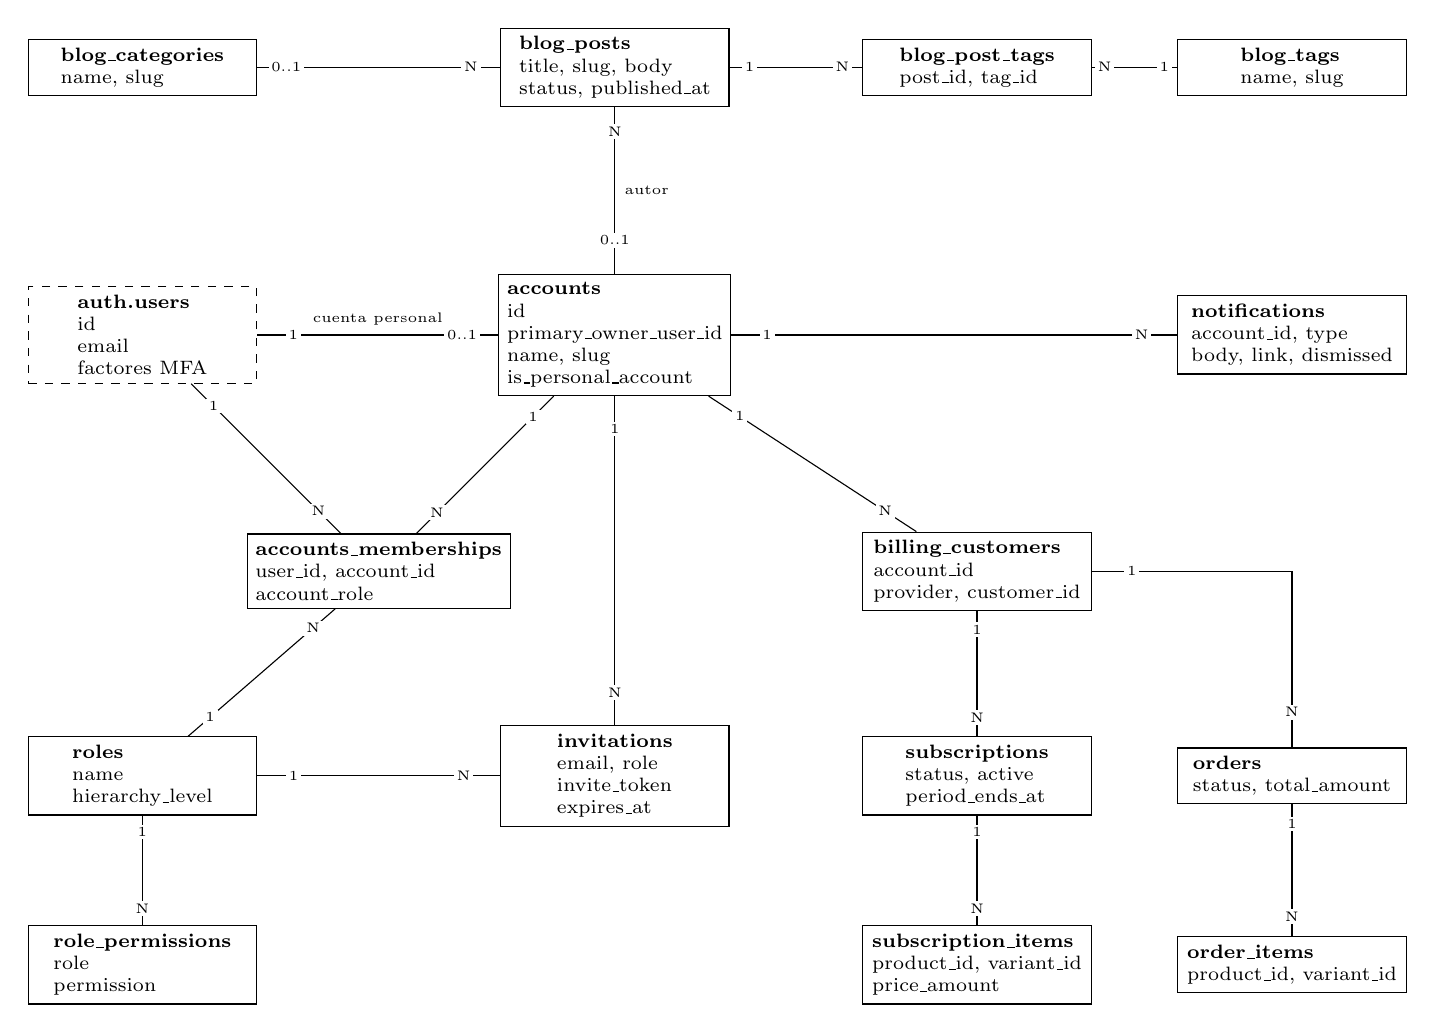
\begin{tikzpicture}[
      font=\scriptsize,
      ent/.style={draw, rectangle, align=left, inner sep=3pt,
                  minimum width=2.9cm, fill=white},
      ext/.style={ent, dashed},
      rel/.style={-},
      card/.style={font=\tiny, inner sep=1pt, fill=white}
    ]
    % Identidad y cuentas
    \node[ext] (users) at (-6, 0) {\textbf{auth.users}\\id\\email\\factores MFA};
    \node[ent] (acc) at (0, 0) {\textbf{accounts}\\id\\primary\_owner\_user\_id\\name, slug\\is\_personal\_account};
    \node[ent] (mem) at (-3, -3) {\textbf{accounts\_memberships}\\user\_id, account\_id\\account\_role};
    \node[ent] (roles) at (-6, -5.6) {\textbf{roles}\\name\\hierarchy\_level};
    \node[ent] (rp) at (-6, -8) {\textbf{role\_permissions}\\role\\permission};
    \node[ent] (inv) at (0, -5.6) {\textbf{invitations}\\email, role\\invite\_token\\expires\_at};

    % Facturación
    \node[ent] (bc) at (4.6, -3) {\textbf{billing\_customers}\\account\_id\\provider, customer\_id};
    \node[ent] (sub) at (4.6, -5.6) {\textbf{subscriptions}\\status, active\\period\_ends\_at};
    \node[ent] (si) at (4.6, -8) {\textbf{subscription\_items}\\product\_id, variant\_id\\price\_amount};
    \node[ent] (ord) at (8.6, -5.6) {\textbf{orders}\\status, total\_amount};
    \node[ent] (oi) at (8.6, -8) {\textbf{order\_items}\\product\_id, variant\_id};

    % Notificaciones
    \node[ent] (not) at (8.6, 0) {\textbf{notifications}\\account\_id, type\\body, link, dismissed};

    % Blog
    \node[ent] (bp) at (0, 3.4) {\textbf{blog\_posts}\\title, slug, body\\status, published\_at};
    \node[ent] (bcat) at (-6, 3.4) {\textbf{blog\_categories}\\name, slug};
    \node[ent] (bpt) at (4.6, 3.4) {\textbf{blog\_post\_tags}\\post\_id, tag\_id};
    \node[ent] (btag) at (8.6, 3.4) {\textbf{blog\_tags}\\name, slug};

    % Relaciones
    \draw[rel] (users) -- node[card, pos=0.15]{1} node[card, pos=0.85]{0..1} node[above, font=\tiny, pos=0.5]{cuenta personal} (acc);
    \draw[rel] (users) -- node[card, pos=0.15]{1} node[card, pos=0.85]{N} (mem);
    \draw[rel] (acc) -- node[card, pos=0.15]{1} node[card, pos=0.85]{N} (mem);
    \draw[rel] (mem) -- node[card, pos=0.15]{N} node[card, pos=0.85]{1} (roles);
    \draw[rel] (roles) -- node[card, pos=0.15]{1} node[card, pos=0.85]{N} (rp);
    \draw[rel] (acc) -- node[card, pos=0.1]{1} node[card, pos=0.9]{N} (inv);
    \draw[rel] (inv.west) -- node[card, pos=0.15]{N} node[card, pos=0.85]{1} (roles.east |- inv.west);
    \draw[rel] (acc) -- node[card, pos=0.15]{1} node[card, pos=0.85]{N} (bc);
    \draw[rel] (bc) -- node[card, pos=0.15]{1} node[card, pos=0.85]{N} (sub);
    \draw[rel] (sub) -- node[card, pos=0.15]{1} node[card, pos=0.85]{N} (si);
    \draw[rel] (bc.east) -| node[card, pos=0.1]{1} node[card, pos=0.9]{N} (ord.north);
    \draw[rel] (ord) -- node[card, pos=0.15]{1} node[card, pos=0.85]{N} (oi);
    \draw[rel] (acc) -- node[card, pos=0.08]{1} node[card, pos=0.92]{N} (not);
    \draw[rel] (bp) -- node[card, pos=0.15]{N} node[card, pos=0.8]{0..1} node[right, font=\tiny, pos=0.5]{autor} (acc);
    \draw[rel] (bp) -- node[card, pos=0.12]{N} node[card, pos=0.88]{0..1} (bcat);
    \draw[rel] (bp) -- node[card, pos=0.15]{1} node[card, pos=0.85]{N} (bpt);
    \draw[rel] (bpt) -- node[card, pos=0.15]{N} node[card, pos=0.85]{1} (btag);
  \end{tikzpicture}}
  \caption{Modelo conceptual de las entidades de la plataforma (esquema
    \texttt{public}). La entidad de trazo discontinuo pertenece al servicio
    de autenticación.}
  \label{fig:ana-datos-public}
  % Texto alternativo: la cuenta (accounts) es el centro del modelo. Cada
  % usuario de auth.users tiene a lo sumo una cuenta personal con su mismo
  % identificador y puede pertenecer a varias cuentas mediante
  % accounts_memberships, que asigna un rol (roles) con sus permisos
  % (role_permissions). Las cuentas tienen invitaciones (con un rol),
  % notificaciones y clientes de facturación, de los que cuelgan
  % suscripciones con sus líneas y pedidos con sus líneas. Las entradas del
  % blog tienen una categoría opcional, un autor (cuenta) opcional y varias
  % etiquetas a través de blog_post_tags.
\end{figure}

La \textbf{cuenta} (\texttt{accounts}) es la unidad de aislamiento
(\textit{tenant}): toda entidad de negocio se enlaza a ella mediante una
columna \texttt{account\_id}. Una cuenta es personal (una por usuario, con su
mismo identificador) o de equipo (con un propietario principal y varios
miembros). Los roles forman una jerarquía mediante
\texttt{hierarchy\_level} y cada uno tiene un conjunto de permisos por
funcionalidad (\texttt{roles.manage}, \texttt{billing.manage},
\texttt{settings.manage}, \texttt{members.manage} e \texttt{invites.manage}).
Por defecto hay tres roles: propietario (\textit{owner}), con todos los
permisos; encargado (\textit{manager}), que gestiona al personal y las
invitaciones pero no la facturación; y miembro (\textit{member}) (ADR-024).
El contenido del blog es la única información pensada para lectura
anónima.

\begin{figure}[htbp]
  \centering
  \resizebox{\textwidth}{!}{%
  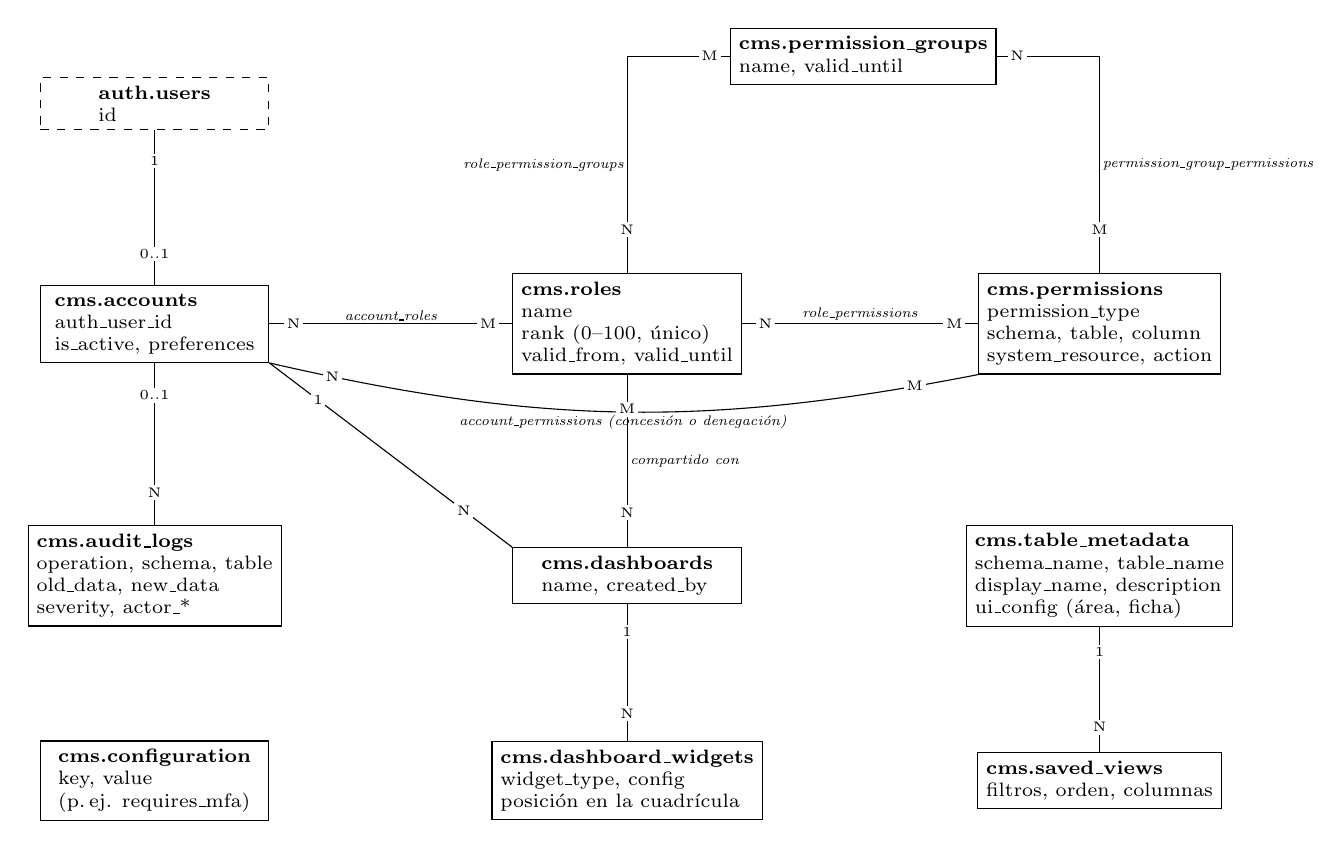
\begin{tikzpicture}[
      font=\scriptsize,
      ent/.style={draw, rectangle, align=left, inner sep=3pt,
                  minimum width=2.9cm, fill=white},
      ext/.style={ent, dashed},
      rel/.style={-},
      card/.style={font=\tiny, inner sep=1pt, fill=white},
      lab/.style={font=\tiny\itshape, fill=white, inner sep=1pt}
    ]
    \node[ext] (users) at (-6, 2.8) {\textbf{auth.users}\\id};
    \node[ent] (cacc) at (-6, 0) {\textbf{cms.accounts}\\auth\_user\_id\\is\_active, preferences};
    \node[ent] (croles) at (0, 0) {\textbf{cms.roles}\\name\\rank (0--100, único)\\valid\_from, valid\_until};
    \node[ent] (cperm) at (6, 0) {\textbf{cms.permissions}\\permission\_type\\schema, table, column\\system\_resource, action};
    \node[ent] (cgroups) at (3, 3.4) {\textbf{cms.permission\_groups}\\name, valid\_until};
    \node[ent] (audit) at (-6, -3.2) {\textbf{cms.audit\_logs}\\operation, schema, table\\old\_data, new\_data\\severity, actor\_*};
    \node[ent] (dash) at (0, -3.2) {\textbf{cms.dashboards}\\name, created\_by};
    \node[ent] (widg) at (0, -5.8) {\textbf{cms.dashboard\_widgets}\\widget\_type, config\\posición en la cuadrícula};
    \node[ent] (meta) at (6, -3.2) {\textbf{cms.table\_metadata}\\schema\_name, table\_name\\display\_name, description\\ui\_config (área, ficha)};
    \node[ent] (views) at (6, -5.8) {\textbf{cms.saved\_views}\\filtros, orden, columnas};
    \node[ent] (conf) at (-6, -5.8) {\textbf{cms.configuration}\\key, value\\(p.\,ej. requires\_mfa)};

    \draw[rel] (users) -- node[card, pos=0.2]{1} node[card, pos=0.8]{0..1} (cacc);
    \draw[rel] (cacc) -- node[card, pos=0.1]{N} node[card, pos=0.9]{M} node[lab, above, pos=0.5]{account\_roles} (croles);
    \draw[rel] (croles) -- node[card, pos=0.1]{N} node[card, pos=0.9]{M} node[lab, above, pos=0.5]{role\_permissions} (cperm);
    \draw[rel] (croles.north) |- node[card, pos=0.1]{N} node[card, pos=0.9]{M} node[lab, pos=0.25, left]{role\_permission\_groups} (cgroups.west);
    \draw[rel] (cgroups.east) -| node[card, pos=0.1]{N} node[card, pos=0.9]{M} node[lab, pos=0.75, right]{permission\_group\_permissions} (cperm.north);
    \draw[rel] (cacc.south east) to[bend right=12] node[card, pos=0.08]{N} node[card, pos=0.92]{M}
      node[lab, below, pos=0.5]{account\_permissions (concesión o denegación)} (cperm.south west);
    \draw[rel] (audit) -- node[card, pos=0.2]{N} node[card, pos=0.8]{0..1} (cacc);
    \draw[rel] (dash.north west) -- node[card, pos=0.2]{N} node[card, pos=0.8]{1} (cacc.south east);
    \draw[rel] (dash) -- node[card, pos=0.2]{1} node[card, pos=0.8]{N} (widg);
    \draw[rel] (dash.north) -- node[card, pos=0.2]{N} node[card, pos=0.8]{M} node[lab, right, pos=0.5]{compartido con} (croles.south);
    \draw[rel] (meta) -- node[card, pos=0.2]{1} node[card, pos=0.8]{N} (views);
  \end{tikzpicture}}
  \caption{Modelo conceptual del esquema \texttt{cms}: control de acceso del
    personal, auditoría, paneles y metadatos de las tablas administradas.}
  \label{fig:ana-datos-cms}
  % Texto alternativo: cada usuario puede tener una cuenta del CMS. Las
  % cuentas tienen roles (con rango único) y los roles tienen permisos,
  % directamente o mediante grupos de permisos; además, una cuenta puede
  % recibir concesiones o denegaciones individuales. La auditoría, los
  % paneles (con sus widgets y compartidos con roles) y las vistas guardadas
  % se relacionan con las cuentas y con los metadatos de tabla, que guardan
  % el nombre visible, la descripción, el área de navegación y el diseño de
  % la ficha de cada tabla. La configuración guarda opciones globales, como
  % la obligatoriedad del MFA.
\end{figure}

El esquema \texttt{cms} añade un segundo modelo de autorización, pensado para
el personal y no para los clientes. Sus permisos son de tres clases:
\emph{de datos} (acción sobre un esquema, una tabla o una columna, con
comodines), \emph{de sistema} (por ejemplo, gestionar miembros o
configuración) y \emph{de almacenamiento} (por contenedor y prefijo de
ruta). Los roles tienen un rango único entre 0 y 100, y todos los permisos,
roles y grupos pueden tener un periodo de vigencia. Los metadatos de tabla
(\texttt{cms.table\_metadata}) son el mecanismo de reutilización del CMS: el
nombre visible, la descripción, el área de la barra lateral y el diseño de
la ficha de cada tabla son \emph{datos}, no código, y se cambian desde la
propia consola (ADR-020).

% ---------------------------------------------------------------------
\section{Reglas de negocio}
\label{sec:ana-reglas}

La tabla~\ref{tab:ana-reglas} recoge las reglas de negocio que el sistema
aplica. Todas se hacen cumplir en la base de datos (restricciones,
\textit{triggers}, políticas o funciones), además de en la interfaz cuando
procede, y cada una está cubierta por pruebas pgTAP.

{\footnotesize
\begin{longtable}{@{}l>{\raggedright\arraybackslash}p{11.4cm}l@{}}
  \caption{Reglas de negocio.}\label{tab:ana-reglas}\\
  \toprule
  \textbf{ID} & \textbf{Regla} & \textbf{Req.} \\
  \midrule
  \endfirsthead
  \toprule
  \textbf{ID} & \textbf{Regla} & \textbf{Req.} \\
  \midrule
  \endhead
  \bottomrule
  \endfoot
  RN-01 & Cada usuario tiene exactamente una cuenta personal, con su mismo identificador. & RF-05 \\
  RN-02 & Una cuenta de equipo tiene un único propietario principal, que solo cambia mediante una transferencia explícita de la propiedad. & RF-06 \\
  RN-03 & El \textit{slug} de una cuenta de equipo y el de una entrada del blog son únicos. & RF-06, RF-09 \\
  RN-04 & Un miembro no puede invitar, asignar ni modificar un rol de nivel superior al suyo. & RF-06 \\
  RN-05 & Las escrituras destructivas (borrar invitaciones, expulsar miembros, gestionar la facturación) exigen el permiso correspondiente, no la mera pertenencia a la cuenta. & RF-06, RNF-02 \\
  RN-06 & Una invitación caduca a los siete días; cada cuenta puede crear como máximo 20 invitaciones por hora y tener 50 pendientes. & RF-06 \\
  RN-07 & Los datos de suscripciones y pedidos solo los escribe la sincronización con la pasarela de pago; ningún usuario los modifica con su sesión. & RF-07 \\
  RN-08 & La consola de administración y el CMS exigen sesión con segundo factor (\texttt{aal2}). & RF-08, RF-09 \\
  RN-09 & Un super-administrador es automáticamente la raíz del CMS (rol de rango máximo); solo existe un rol raíz y retirar la condición de super-administrador retira el acceso, conservando la cuenta para la auditoría. & RF-08, RF-09 \\
  RN-10 & En el CMS nadie actúa sobre su propia cuenta ni sobre cuentas de rango igual o superior, y las cuentas raíz no se desactivan ni pierden su rol desde la consola. & RF-09 \\
  RN-11 & Una denegación explícita prevalece sobre cualquier concesión, y solo se puede delegar un permiso que se tiene y que no se solapa con ninguna denegación propia. & RF-09, RNF-02 \\
  RN-12 & El MFA del CMS es obligatorio por defecto; solo una cuenta raíz con sesión \texttt{aal2} puede desactivarlo, y el cambio queda auditado. & RF-09, RF-10 \\
  RN-13 & La auditoría solo la escriben las funciones del sistema, con el autor tomado de la sesión; una escritura cuya auditoría falla se deshace. & RF-10 \\
  RN-14 & La auditoría conserva una instantánea del autor aunque se borre su cuenta (ADR-018). & RF-10 \\
  RN-15 & Un \textit{widget} de un panel solo muestra datos de tablas que puede leer quien lo ve, aunque el panel esté compartido. & RF-11 \\
  RN-16 & En la web pública solo es visible una entrada del blog publicada cuya fecha de publicación ya se ha alcanzado. & RF-01 \\
  RN-17 & Los esquemas del sistema (\texttt{auth}, catálogos de PostgreSQL y otros protegidos) nunca se exploran ni se buscan desde el CMS. & RF-09, RNF-02 \\
\end{longtable}}



\chapter{Diseño del Sistema}
% =====================================================================
% Capítulo: Diseño del Sistema
% Fuentes: borradores/05-diseno.tex, docs/tfg/DECISIONES.md (ADR-001…021),
% AGENTS.md, apps/web/AGENTS.md, apps/web/supabase/AGENTS.md,
% apps/web/src/config/*.config.ts, packages/cms/*,
% packages/function-middleware. Estado de las fuentes: F3c cerrada.
% =====================================================================

Este capítulo describe el diseño de PymeKit: la arquitectura general, el
modelo multi-tenant y de control de acceso, la estrategia de seguridad en
profundidad, la integración con la pasarela de pago, el diseño de la interfaz
y los mecanismos de configuración que hacen la plataforma reutilizable. Cada
decisión remite al registro de decisiones de arquitectura (ADR,
\textit{Architecture Decision Record}~\cite{nygard2011adr}) del proyecto, que
se resume en la sección~\ref{sec:dis-decisiones}. La infraestructura de
ejecución (contenedores, nube y puesta en marcha) se trata en el capítulo de
Despliegue del Sistema.

% ---------------------------------------------------------------------
\section{Arquitectura general}
\label{sec:dis-arquitectura}

\subsection{Monorepo de paquetes}
\label{sec:dis-monorepo}

El código se organiza en un único \textit{monorepo} (un repositorio con
varias aplicaciones y paquetes que se versionan juntos) gestionado con
Turborepo~\cite{turborepo} y pnpm (ADR-002):

\begin{itemize}
  \item \texttt{apps/web}: la aplicación web, que incluye la web pública, el
        área privada, la consola de administración y el CMS;
  \item \texttt{apps/web/supabase}: esquemas, migraciones, datos de prueba y
        pruebas pgTAP de \emph{toda} la base de datos;
  \item \texttt{apps/e2e}: las pruebas E2E con Playwright~\cite{playwright};
  \item \texttt{packages/*}: los paquetes reutilizables de la plataforma
        (\texttt{@pymekit/*}: interfaz, cliente de base de datos,
        \textit{middleware}, autenticación, cuentas, equipos, facturación,
        administración, i18n\ldots);
  \item \texttt{packages/cms/*}: los paquetes del CMS
        (\texttt{@pymekit/cms-*}), separados en paquetes de servidor
        (servicios y rutas de la API) y paquetes de cliente (componentes de
        las pantallas).
\end{itemize}

El monorepo contiene 51 paquetes, 27 de ellos del CMS, sin ciclos de
dependencias (RNF-04). Cada paquete declara sus dependencias de forma
explícita y separa las exportaciones de cliente y de servidor. Esta
separación evita que código con credenciales de servidor acabe en el
navegador ---la \textit{build} de la web falla si el cliente de base de datos
del servidor aparece en un fragmento destinado al navegador--- y, como se
comprobó en la incidencia B-16, también evita ciclos entre paquetes.

\subsection{Capas y pila tecnológica}
\label{sec:dis-capas}

La aplicación sigue una arquitectura en capas en la que cada capa solo
depende de la inferior y la base de datos es la última barrera de
autorización:

\begin{enumerate}
  \item \textbf{Presentación.} Rutas por fichero de TanStack
        Router~\cite{tanstack-router} con React 19, renderizadas en el
        servidor (SSR). Componentes accesibles de \texttt{@pymekit/ui}
        con Tailwind CSS. La caché de datos del cliente usa TanStack
        Query~\cite{tanstack-query}.
  \item \textbf{Aplicación.} \textit{Server functions} de TanStack
        Start~\cite{tanstack-start}: funciones que se ejecutan en el servidor
        y se invocan desde el cliente con tipos compartidos, validadas con
        Zod y protegidas por una cadena de \textit{middleware} (RF-02). Para el
        CMS, una API HTTP construida con Hono~\cite{hono}.
  \item \textbf{Servicios.} Lógica de negocio en servicios sin dependencia de
        la interfaz, con el cliente de datos inyectado: el cliente de
        Supabase~\cite{supabase-docs} en la web y Drizzle ORM~\cite{drizzle}
        en el CMS.
  \item \textbf{Datos.} PostgreSQL con políticas de seguridad a nivel de fila
        (RLS), funciones y \textit{triggers}; servicio de autenticación con
        JWT y MFA; almacenamiento de ficheros.
\end{enumerate}

Para que el conjunto sea coherente se usa una sola pila de librerías en toda
la web, CMS incluido: un único sistema de formularios, uno de
internacionalización y una sola biblioteca de componentes (ADR-013). Así cada
cosa se hace de una única forma (RNF-05).

\subsection{Una única base de datos}
\label{sec:dis-bd-unica}

La aplicación y el CMS comparten \textbf{una sola instancia} de PostgreSQL
(ADR-002). Los datos de la plataforma viven en el esquema \texttt{public} y
los del CMS en un esquema propio, \texttt{cms} (ADR-012). Compartir la base de
datos es lo que permite que el CMS administre los datos de la propia
plataforma ---incluido el blog que publica la web (ADR-017)--- y que las
mismas políticas de seguridad protejan ambas partes. Los esquemas
declarativos se numeran (del \texttt{00} al \texttt{55}) para fijar el orden
de creación, y las migraciones se generan a partir de ellos.

\subsection{CMS integrado en la consola de administración}
\label{sec:dis-cms-integrado}

La decisión de mayor calado del diseño es cómo integrar el CMS (ADR-011). Un
CMS de este tipo se construye habitualmente como una aplicación de página
única con su propio enrutador y una API independiente. Se evaluaron tres opciones:

\begin{enumerate}[label=(\alph*)]
  \item \textbf{aplicaciones separadas} (la web, la interfaz del CMS y su
        API como tres servicios): la de menor esfuerzo, pero con tres
        despliegues, dos inicios de sesión y las \textit{cookies} de sesión
        duplicadas;
  \item \textbf{integración híbrida} (la API dentro de la web y la interfaz
        del CMS servida como aplicación estática): convivirían dos
        enrutadores y dos formas de programar;
  \item \textbf{integración total}: la API se monta dentro del servidor de
        la web y las pantallas se reescriben como rutas de la web.
\end{enumerate}

Se eligió la opción (c), aun siendo la de mayor esfuerzo estimado, porque da
un único servicio, un único inicio de sesión y un único estilo de código:

\begin{itemize}
  \item La aplicación Hono del CMS se monta en \texttt{/api/cms/*} mediante
        una ruta de servidor de la web que le reenvía la petición tal cual.
        El CMS comparte así proceso, dominio y \textit{cookies} con la web.
  \item Las pantallas del CMS son rutas de la web bajo \texttt{/admin/cms/*},
        con \textit{loaders} y TanStack Query sobre un cliente RPC tipado de
        la API.
  \item Durante el SSR, los \textit{loaders} no hacen una petición de red a la
        propia API: invocan la aplicación Hono dentro del mismo proceso,
        reenviando solo la cabecera \texttt{cookie} (ADR-016).
\end{itemize}

La figura~\ref{fig:dis-arquitectura} resume la arquitectura resultante.

\begin{figure}[htbp]
  \centering
  \resizebox{\textwidth}{!}{%
  \begin{tikzpicture}[
      font=\footnotesize,
      box/.style={draw, rounded corners, align=center, minimum height=0.9cm,
                  inner sep=4pt, fill=white},
      group/.style={draw, dashed, rounded corners, inner sep=8pt},
      arr/.style={-{Stealth[length=2mm]}}
    ]
    \node[box, minimum width=11cm] (browser) at (0, 5.2)
      {Navegador (React 19): web pública, área privada, consola \texttt{/admin} y CMS \texttt{/admin/cms}};

    \node[box, minimum width=3.0cm] (ssr) at (-3.8, 3.3)
      {Rutas y \textit{loaders}\\(SSR, TanStack Router)};
    \node[box, minimum width=3.0cm] (sfn) at (0, 3.3)
      {\textit{Server functions}\\+ \textit{middleware}};
    \node[box, minimum width=3.0cm] (hono) at (3.8, 3.3)
      {Ruta \texttt{/api/cms/*}\\$\rightarrow$ aplicación Hono};
    \node[box, minimum width=3.0cm] (svc) at (-1.9, 1.6)
      {Servicios + cliente Supabase\\(sesión del usuario)};
    \node[box, minimum width=3.0cm] (drizzle) at (3.8, 1.6)
      {Servicios Drizzle\\(\textit{claims} del usuario)};
    \node[box, minimum width=2.4cm] (wh) at (-6.6, 1.6)
      {Ruta \texttt{/api/billing}\\\textit{webhook}};

    \begin{scope}[on background layer]
      \node[group, fit=(ssr)(sfn)(hono)(svc)(drizzle)(wh),
            label={[font=\small\bfseries, anchor=north east]south east:\texttt{apps/web} (TanStack Start, un único proceso)}] (web) {};
    \end{scope}

    \node[box, minimum width=2.6cm] (auth) at (-3.8, -0.6) {Auth\\(JWT, MFA)};
    \node[box, minimum width=4.6cm] (pg) at (0.4, -0.6)
      {PostgreSQL + RLS\\esquemas \texttt{public}, \texttt{cms} y \texttt{auth}};
    \node[box, minimum width=2.2cm] (st) at (4.4, -0.6) {Storage};
    \begin{scope}[on background layer]
      \node[group, fit=(auth)(pg)(st),
            label={[font=\small\bfseries]below:Supabase (una única instancia)}] (sb) {};
    \end{scope}

    \node[box] (stripe) at (-10.6, 1.6) {Pasarela\\de pago};

    \draw[arr] (browser) -- (ssr);
    \draw[arr] (browser) -- (sfn);
    \draw[arr] (browser) -- node[right, font=\scriptsize]{RPC} (hono);
    \draw[arr] (ssr) -- (sfn);
    \draw[arr, dashed] (ssr.south) -- ++(0,-0.3) coordinate (ssrq) -- (ssrq -| hono.south) node[midway, below, font=\scriptsize, fill=white, inner sep=1pt]{SSR en proceso} -- (hono.south);
    \draw[arr] (sfn) -- (svc);
    \draw[arr] (hono) -- (drizzle);
    \draw[arr] (svc) -- (pg);
    \draw[arr] (svc) -- (auth);
    \draw[arr] (drizzle) -- (pg);
    \draw[arr] (stripe) -- node[above, font=\scriptsize]{\textit{webhooks}} (wh);
    \draw[arr] (wh) |- (pg.west);
    \draw[arr, dashed] (sfn.north west) to[bend right=25] node[above, font=\scriptsize, pos=0.6]{\textit{checkout}} (stripe.north);
  \end{tikzpicture}}
  \caption{Arquitectura general de PymeKit: una única aplicación web con el
    CMS integrado y una única instancia de la base de datos.}
  \label{fig:dis-arquitectura}
  % Texto alternativo: el navegador se comunica con la aplicación web, que
  % contiene las rutas con SSR, las server functions y la ruta /api/cms que
  % monta la aplicación Hono del CMS. Las server functions usan servicios con
  % el cliente de Supabase y la sesión del usuario; la API del CMS usa
  % servicios Drizzle con los claims del usuario. Ambos acceden a una única
  % instancia (Auth, PostgreSQL con RLS y Storage). La pasarela de pago
  % recibe las sesiones de pago desde las server functions y notifica los
  % cambios a la ruta de webhook, que actualiza la base de datos.
\end{figure}

% ---------------------------------------------------------------------
\section{Modelo multi-tenant y control de acceso}
\label{sec:dis-multitenant}

\subsection{Cuentas como unidad de aislamiento}
\label{sec:dis-cuentas}

PymeKit sigue un modelo multi-tenant de \emph{base de datos y esquema
compartidos}: todos los clientes comparten tablas y cada fila lleva el
identificador de la cuenta a la que pertenece. Es el modelo de menor coste de
operación y el que más simplifica las actualizaciones, a cambio de que el
aislamiento dependa por completo de la corrección del control de
acceso~\cite{bezemer2010multitenant}. Por eso el diseño traslada ese control a la base de
datos.

El \textit{tenant} es la cuenta (sección~\ref{sec:ana-modelo-datos}). La
relación de un usuario con una cuenta se resuelve con un pequeño conjunto de
funciones auxiliares sobre las que se escriben todas las políticas:
\texttt{has\_role\_on\_account} (pertenencia), \texttt{has\_permission}
(permiso concreto) y \texttt{has\_more\_elevated\_role} (jerarquía). Las
escrituras destructivas se condicionan al permiso, no a la mera pertenencia,
y la cuenta activa de cada sesión se guarda en el servidor
(\texttt{user\_active\_account}) para que el área privada sepa en qué
contexto trabaja el usuario.

El modelo admite tres modos, elegidos por configuración
(sección~\ref{sec:dis-configuracion}): solo cuentas personales (B2C), solo
cuentas de equipo (B2B) o ambas. En la web de una sola pyme (ADR-020), los
equipos pueden representar, por ejemplo, las tiendas de la empresa, y sus
clientes usar la cuenta personal.

\subsection{Control de acceso del CMS}
\label{sec:dis-rbac-cms}

El CMS tiene su propio control de acceso basado en roles
(\textit{Role-Based Access Control}, RBAC) en el esquema \texttt{cms}. Conviven
así dos modelos de autorización en la misma base de datos
(tabla~\ref{tab:dis-dos-modelos}). La decisión de diseño (ADR-014) fue
conectarlos en lugar de sustituir uno por otro:

\begin{itemize}
  \item \textbf{El super-administrador es la raíz del CMS.} Unos
        \textit{triggers} sobre los usuarios sincronizan a los
        super-administradores con un rol de sistema \emph{Root}, de rango
        máximo, que concede todos los permisos. Al promocionar a un usuario
        recibe acceso, una cuenta activa del CMS y ese rol; al retirarle la
        condición pierde el acceso y su cuenta se desactiva, pero se conserva
        para la auditoría. Un índice único garantiza que solo exista un rol
        raíz.
  \item \textbf{El RBAC del CMS da acceso limitado a otro personal}
        (soporte, gestión de contenidos). Se descartó dejar solo al
        super-administrador porque incumpliría RF-09 («con permisos
        propios»). Para que una instalación nueva no empiece con el RBAC
        vacío, una migración de datos idempotente deja preparados dos roles
        de partida, editables y sin nadie asignado (ADR-026): «Soporte»,
        que solo lee cuentas, miembros, usuarios y la auditoría, y «Gestor
        de contenidos», que gestiona el blog y los archivos a través de un
        grupo de permisos «Contenidos». Se eligió una migración y no el
        \textit{seed} porque este solo se aplica en desarrollo.
\end{itemize}

\begin{table}[htbp]
  \centering
  \footnotesize
  \caption{Los dos modelos de autorización de PymeKit.}
  \label{tab:dis-dos-modelos}
  \begin{tabularx}{\textwidth}{@{}>{\raggedright\arraybackslash}p{2.6cm}XX@{}}
    \toprule
     & \textbf{Plataforma (\texttt{public})} & \textbf{CMS (\texttt{cms})} \\
    \midrule
    Sujetos & Usuarios de las cuentas (clientes) & Personal con cuenta del CMS \\
    Ámbito & Una cuenta (\textit{tenant}) & Toda la base de datos administrada \\
    Roles & Jerarquía por \texttt{hierarchy\_level} & Rango único 0--100, con vigencia \\
    Permisos & Cinco permisos por funcionalidad & De datos (esquema, tabla, columna), de sistema y de almacenamiento; grupos; concesiones y denegaciones por cuenta \\
    Raíz & Propietario principal de cada cuenta & Rol Root, ligado al super-administrador \\
    MFA & Exigido si el usuario lo tiene configurado & Obligatorio por defecto \\
    \bottomrule
  \end{tabularx}
\end{table}

\subsection{Acceso a la consola}
\label{sec:dis-acceso-consola}

Super-administradores y personal del CMS comparten la consola, con límites
distintos (ADR-016): la consola admite a quien es super-administrador
\emph{o} tiene acceso al CMS; las páginas de gestión de la plataforma exigen
super-administrador y redirigen al personal al CMS. La barra lateral solo
muestra las secciones que la API permite, pero esa ocultación es solo de
interfaz: cada ruta y cada \textit{endpoint} vuelven a comprobar el permiso.

% ---------------------------------------------------------------------
\section{Seguridad en profundidad}
\label{sec:dis-seguridad}

El principio que guía el diseño es que \textbf{la base de datos es la
frontera de autorización} (RNF-02): toda comprobación en la interfaz o en el
servidor de aplicación es una primera barrera, útil para la experiencia de
uso, pero nunca suficiente. Si una capa superior falla, las políticas de la
base de datos siguen impidiendo el acceso, en línea con las recomendaciones
de verificación de seguridad de OWASP~\cite{owasp-asvs}.

\subsection{RLS como frontera}
\label{sec:dis-rls}

PostgreSQL permite asociar a cada tabla políticas de seguridad a nivel de
fila (\textit{Row-Level Security}, RLS)~\cite{postgresql-rls}: predicados que
el propio motor añade a cada consulta según el usuario que la ejecuta.
Supabase~\cite{supabase-rls} traslada la identidad del usuario (su JWT) a la
sesión de PostgreSQL, de modo que las políticas deciden con ella. Las reglas
de diseño, recogidas en las directrices de la base de datos, son:

\begin{itemize}
  \item RLS activo en toda tabla. Se revocan los privilegios por defecto a
        los tres roles de la API (\texttt{anon}, \texttt{authenticated} y
        \texttt{service\_role}), incluidos los que ignoran RLS como
        \texttt{TRUNCATE}, y se conceden solo los verbos que la funcionalidad
        usa.
  \item El \texttt{UPDATE} se concede por columnas, dejando fuera las de
        identidad y de pertenencia (\texttt{id}, \texttt{account\_id}), para
        que nadie pueda mover una fila a otra cuenta.
  \item Las políticas de \texttt{UPDATE} repiten en \texttt{WITH CHECK} las
        comprobaciones del \texttt{INSERT}: sin esa cláusula PostgreSQL solo
        valida la fila antigua~\cite{postgresql-createpolicy} (B-05, B-50).
  \item Toda función \texttt{security definer}, que se ejecuta con
        privilegios elevados y se salta RLS, aplica sus propias
        comprobaciones y las justifica en un comentario; las funciones
        internas no son ejecutables por los roles de la API (B-45).
  \item Las llamadas a funciones dentro de un predicado se envuelven en
        \texttt{(select \ldots)} para que se evalúen una sola vez (B-55).
  \item El cliente de servidor que ignora RLS se reserva para casos
        excepcionales, tras validar a mano los permisos.
\end{itemize}

\subsection{Segundo factor obligatorio en la administración}
\label{sec:dis-mfa}

El servicio de autenticación distingue el nivel de garantía de la sesión
(\textit{Authenticator Assurance Level}, AAL)~\cite{supabase-mfa}:
\texttt{aal1} tras la contraseña y \texttt{aal2} tras completar el segundo
factor. El diseño exige \texttt{aal2} en todas las capas que dan acceso a la
administración:

\begin{itemize}
  \item en la base de datos, la función que identifica al super-administrador
        devuelve falso si la sesión no es \texttt{aal2}; unas políticas
        restrictivas exigen \texttt{aal2} a quien tiene un factor
        configurado; y el acceso al CMS lo decide
        \texttt{cms.verify\_admin\_access()}, que comprueba la cuenta activa
        del CMS y el MFA;
  \item en la interfaz, la consola exige siempre \texttt{aal2}: con un factor
        configurado redirige a la verificación y vuelve a la página pedida;
        sin factor responde 404 (ADR-016).
\end{itemize}

\subsection{Middleware más comprobación en la base de datos}
\label{sec:dis-middleware}

La figura~\ref{fig:dis-flujo-cms} muestra el recorrido de una petición a la
API del CMS y las comprobaciones que encuentra en cada capa. Las
\textit{server functions} de la web siguen el mismo patrón: una cadena de
\textit{middleware} tipado (autenticación, pertenencia al equipo, permiso por
funcionalidad, super-administrador) valida la petición y después el cliente de
Supabase con la sesión del usuario deja que RLS tome la decisión final.

\begin{figure}[htbp]
  \centering
  \resizebox{\textwidth}{!}{%
  \begin{tikzpicture}[
      font=\footnotesize,
      paso/.style={draw, rounded corners, align=center, minimum width=3.3cm,
                   minimum height=1.0cm, inner sep=3pt},
      check/.style={align=left, font=\scriptsize, text width=7.6cm},
      arr/.style={-{Stealth[length=2mm]}}
    ]
    \node[paso] (s1) at (0, 0)     {Navegador\\(consola \texttt{/admin/cms})};
    \node[paso] (s2) at (0, -1.6)  {Ruta de servidor\\\texttt{/api/cms/\$}};
    \node[paso] (s3) at (0, -3.2)  {Aplicación Hono\\(\textit{middleware})};
    \node[paso] (s4) at (0, -4.8)  {Servicio Drizzle\\(transacción)};
    \node[paso] (s5) at (0, -6.4)  {PostgreSQL\\(esquema \texttt{cms})};

    \draw[arr] (s1) -- (s2);
    \draw[arr] (s2) -- (s3);
    \draw[arr] (s3) -- (s4);
    \draw[arr] (s4) -- (s5);

    \node[check, right=0.6cm of s1] {Guarda de ruta: sesión viva y
      \texttt{aal2}, acceso de administración (si no: inicio de sesión,
      verificación MFA o 404)};
    \node[check, right=0.6cm of s2] {Reenvío a Hono; el código del CMS se
      importa solo en el servidor};
    \node[check, right=0.6cm of s3] {Cabeceras de seguridad y CSRF propia; JWT
      válido (401), acceso al CMS (403), usuario no bloqueado (en cerrado);
      validación estricta de la entrada con Zod (400)};
    \node[check, right=0.6cm of s4] {\textit{Claims} del usuario y rol
      \texttt{authenticated} fijados con parámetros enlazados; permiso
      concreto comprobado por el servicio};
    \node[check, right=0.6cm of s5] {\texttt{cms.verify\_admin\_access()}
      (cuenta activa, MFA) y políticas RLS: \textbf{decisión final}};
  \end{tikzpicture}}
  \caption{Flujo de una petición a la API del CMS y comprobaciones de
    seguridad en cada capa.}
  \label{fig:dis-flujo-cms}
  % Texto alternativo: diagrama vertical de cinco pasos (navegador, ruta de
  % servidor, aplicación Hono, servicio Drizzle, PostgreSQL). A la derecha de
  % cada paso se indican sus comprobaciones; la última, la base de datos, es
  % la que toma la decisión.
\end{figure}

Dos detalles del diseño merecen mención. Primero, el servicio fija la
identidad del usuario en la transacción mediante parámetros enlazados, nunca
interpolando valores del JWT en el SQL, de modo que las políticas RLS del
esquema \texttt{cms} se aplican igual que a cualquier otro cliente. Segundo,
un super-administrador con sesión \texttt{aal1} supera el \textit{middleware}
(tiene el \textit{claim} de acceso), pero no ve datos, porque la base de
datos exige el segundo factor: es la defensa en profundidad en acción.

\subsection{Fallo en cerrado y errores sin detalles internos}
\label{sec:dis-fallo-cerrado}

Todas las comprobaciones de seguridad \textbf{fallan en cerrado}
(\textit{fail closed}): ante un dato ausente, ilegible o no válido, se
deniega. El diseño lo aplica a la opción que indica si el CMS exige MFA, que
se lee con una función de privilegios elevados para que RLS no pueda
ocultársela a quien decide (B-06); a la comprobación de usuario bloqueado
cuando el servicio de autenticación no responde (B-23); y a la auditoría,
cuyo fallo deshace la escritura auditada (B-41).

Del mismo modo, los errores de la base de datos se clasifican en el servidor:
el cliente solo recibe un estado HTTP y un código estable
(\texttt{RECORD\_*}, \texttt{SETTINGS\_*}, \texttt{AUDIT\_LOG\_*}\ldots),
nunca el texto de PostgreSQL, que podría revelar nombres de tablas o
restricciones (B-20, B-33).

\subsection{Seguridad del entorno de desarrollo}
\label{sec:dis-seguridad-entorno}

La seguridad alcanza también al entorno de trabajo. Los servicios locales de
la base de datos se aíslan de Internet con una regla de cortafuegos específica
para contenedores y la aplicación se consulta mediante un túnel SSH (ADR-010,
tras la incidencia B-04). Los secretos nunca se versionan.

% ---------------------------------------------------------------------
\section{Integración con la pasarela de pago}
\label{sec:dis-pagos}

La facturación se diseña detrás de una \emph{pasarela abstracta}
(\path{@pymekit/billing-gateway}) con una estrategia por proveedor: la
aplicación pide «crear una sesión de pago» o «abrir el portal de cliente» sin
conocer el proveedor concreto, que se elige con la variable
\path{VITE_BILLING_PROVIDER} y se valida al construir la aplicación.
Actualmente se registra Stripe.

Los planes, sus precios y sus características se declaran en
\path{billing.config.ts}, validado con un esquema. El flujo tiene dos
sentidos (figura~\ref{fig:dis-arquitectura}): las \textit{server functions}
crean la sesión de pago tras comprobar el permiso \texttt{billing.manage}; y
la pasarela notifica cada cambio a la ruta \texttt{/api/billing/webhook}, que
verifica la firma y sincroniza clientes, suscripciones y pedidos con el
cliente de servicio. Ningún usuario escribe esas tablas con su sesión
(RN-07): la fuente de verdad de un cobro es la pasarela.

Los planes de partida están pensados para una pyme (ADR-025): «Básico»,
«Profesional» y «Empresa», en euros, cada uno con pago mensual y anual. Los
importes son ficticios y los identificadores de precio de la pasarela se
leen de variables de entorno (\texttt{VITE\_STRIPE\_PRICE\_*}); si faltan,
se usan valores de relleno marcados como ejemplo, de modo que la página de
precios funciona desde el primer arranque y la pyme solo tiene que crear sus
precios en Stripe y copiar sus identificadores. Los textos de cada plan son
claves de traducción.

El flujo completo se verificó con una cuenta de Stripe en modo de pruebas:
los planes se crearon en la pasarela con sus importes en euros, la CLI de
Stripe reenvió los avisos de pago a la aplicación local sin necesidad de una
URL pública, y las pruebas E2E de facturación de equipo y personal pagaron
con la tarjeta de prueba y comprobaron que la suscripción quedaba activa en
la aplicación tras recibir \texttt{checkout.session.completed} e
\texttt{invoice.paid}. Las pruebas heredadas suponían una cuenta con solo
pago con tarjeta y hubo que adaptarlas a una cuenta europea, que ofrece
varios métodos de pago (B-62).

% ---------------------------------------------------------------------
\section{Diseño de la interfaz}
\label{sec:dis-interfaz}

\subsection{Web pública y área privada}

La web pública ofrece inicio, precios, blog, preguntas frecuentes, contacto y
textos legales (plantillas con los apartados que exigen el RGPD y la LSSI-CE,
que cada pyme completa con sus datos); el área privada, el panel de la cuenta activa, sus ajustes,
miembros y facturación. La identidad visual es propia (logotipo, iconos y
capturas generadas a partir de la propia aplicación, B-46). La interfaz es
adaptable a dispositivos móviles, admite tema claro y oscuro y se construye
con componentes accesibles (RNF-08).

Mientras PymeKit se presenta como TFG, la página de inicio incluye un bloque
académico (logotipo de la escuela, autor, tutor y un recorrido guiado por la
demostración). Depende de un único interruptor de configuración, de modo que
una pyme que reutilice la plataforma lo desactiva sin tocar el código
(sección~\ref{sec:dis-configuracion}).

\subsection{Consola de administración por áreas de negocio}
\label{sec:dis-consola}

La primera versión de la consola separaba «Plataforma», «CMS» y «Recursos» y
agrupaba las tablas por esquema SQL, una organización técnica que no entiende
quien gestiona una pyme. Tras la revisión del autor se rediseñó como una
\textbf{única consola organizada por áreas de negocio} (ADR-020,
figura~\ref{fig:dis-consola}):

\begin{itemize}
  \item un bloque \textbf{Gestión} con Inicio, Gestión de cuentas (solo
        super-administrador) y las herramientas del CMS: Usuarios, Archivos,
        Paneles, Auditoría y Ajustes;
  \item un bloque \textbf{Datos} con una entrada plegable por área (Blog,
        Cuentas, Facturación, Sistema y Otros datos) que contiene sus tablas
        con nombre en español, y una entrada «Todas las tablas».
\end{itemize}

El área de cada tabla, su nombre visible y su descripción son \emph{datos}
de los metadatos del CMS, editables en Ajustes $\rightarrow$ Recursos, de
modo que una pyme puede crear áreas para sus propias tablas sin programar.
Las tablas de esquemas protegidos no aparecen en la navegación.

\begin{figure}[htbp]
  \centering
  \begin{subfigure}{\textwidth}
    \centering
    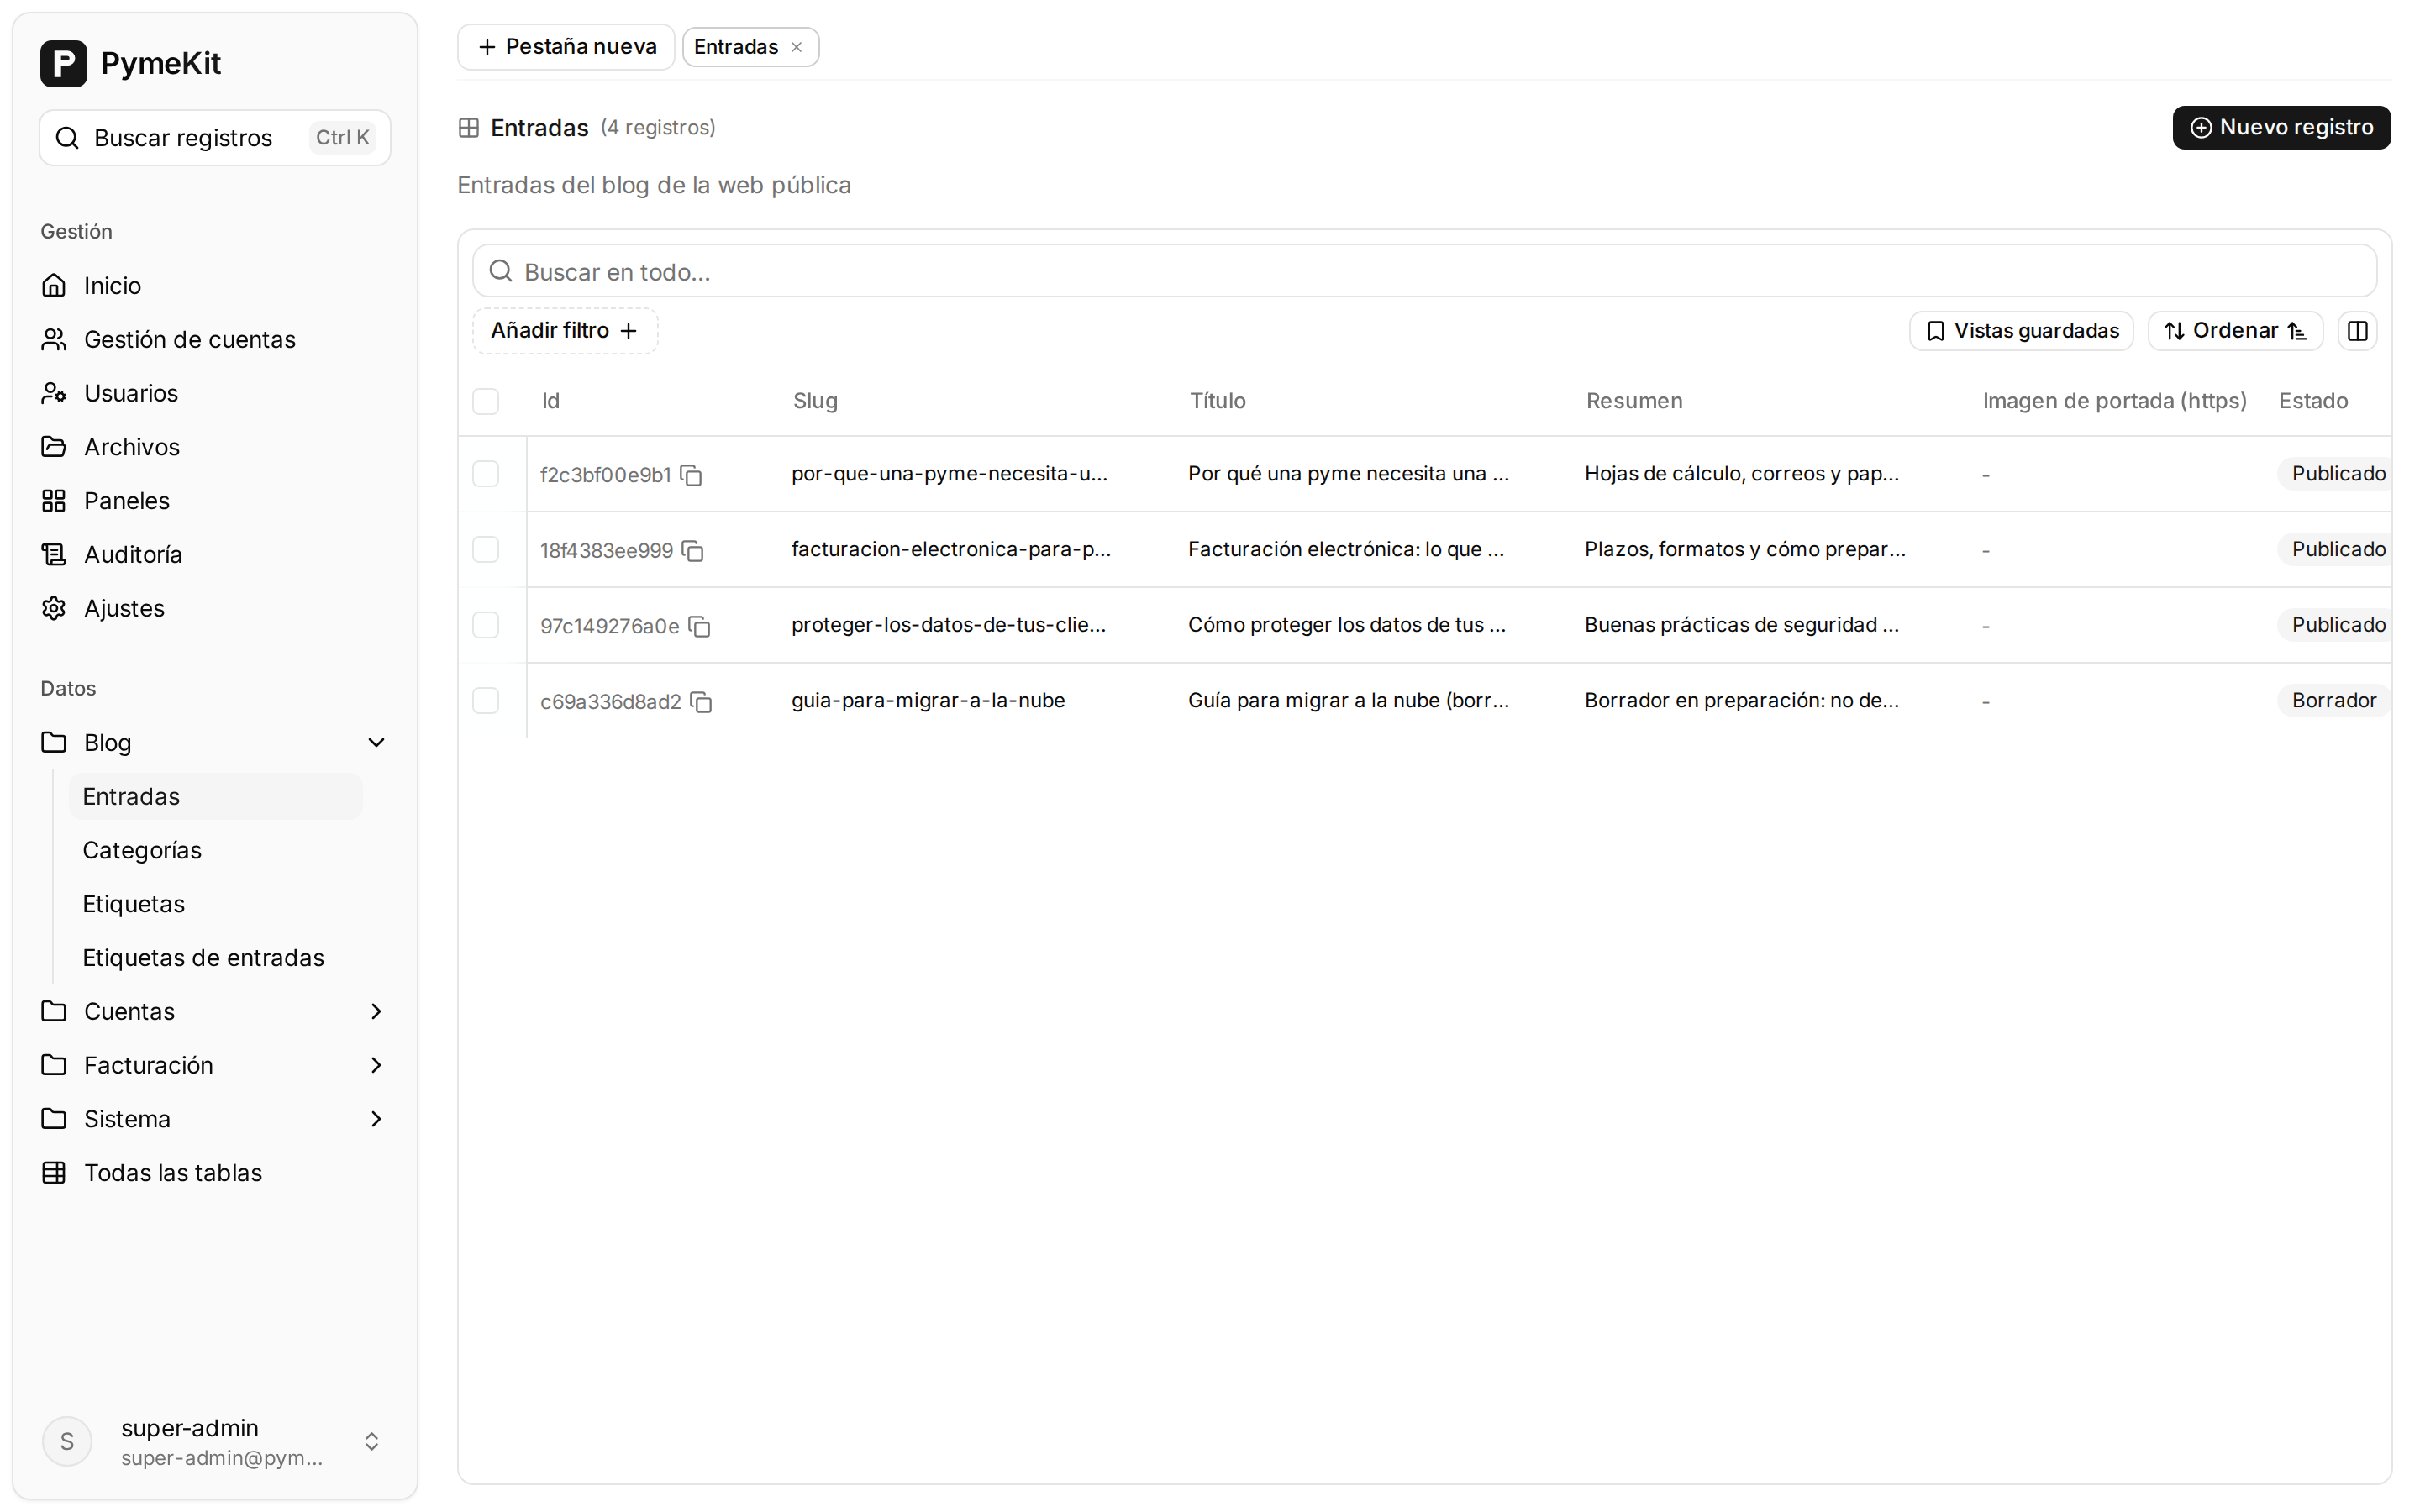
\includegraphics[width=0.92\textwidth]{figures/consola-explorador.png}
    \caption{Barra lateral con los bloques «Gestión» y «Datos» (área «Blog»
      desplegada) y listado de las entradas del blog con el resumen de la
      tabla bajo el título.}
    \label{fig:dis-consola-explorador}
  \end{subfigure}

  \vspace{0.6cm}
  \begin{subfigure}{\textwidth}
    \centering
    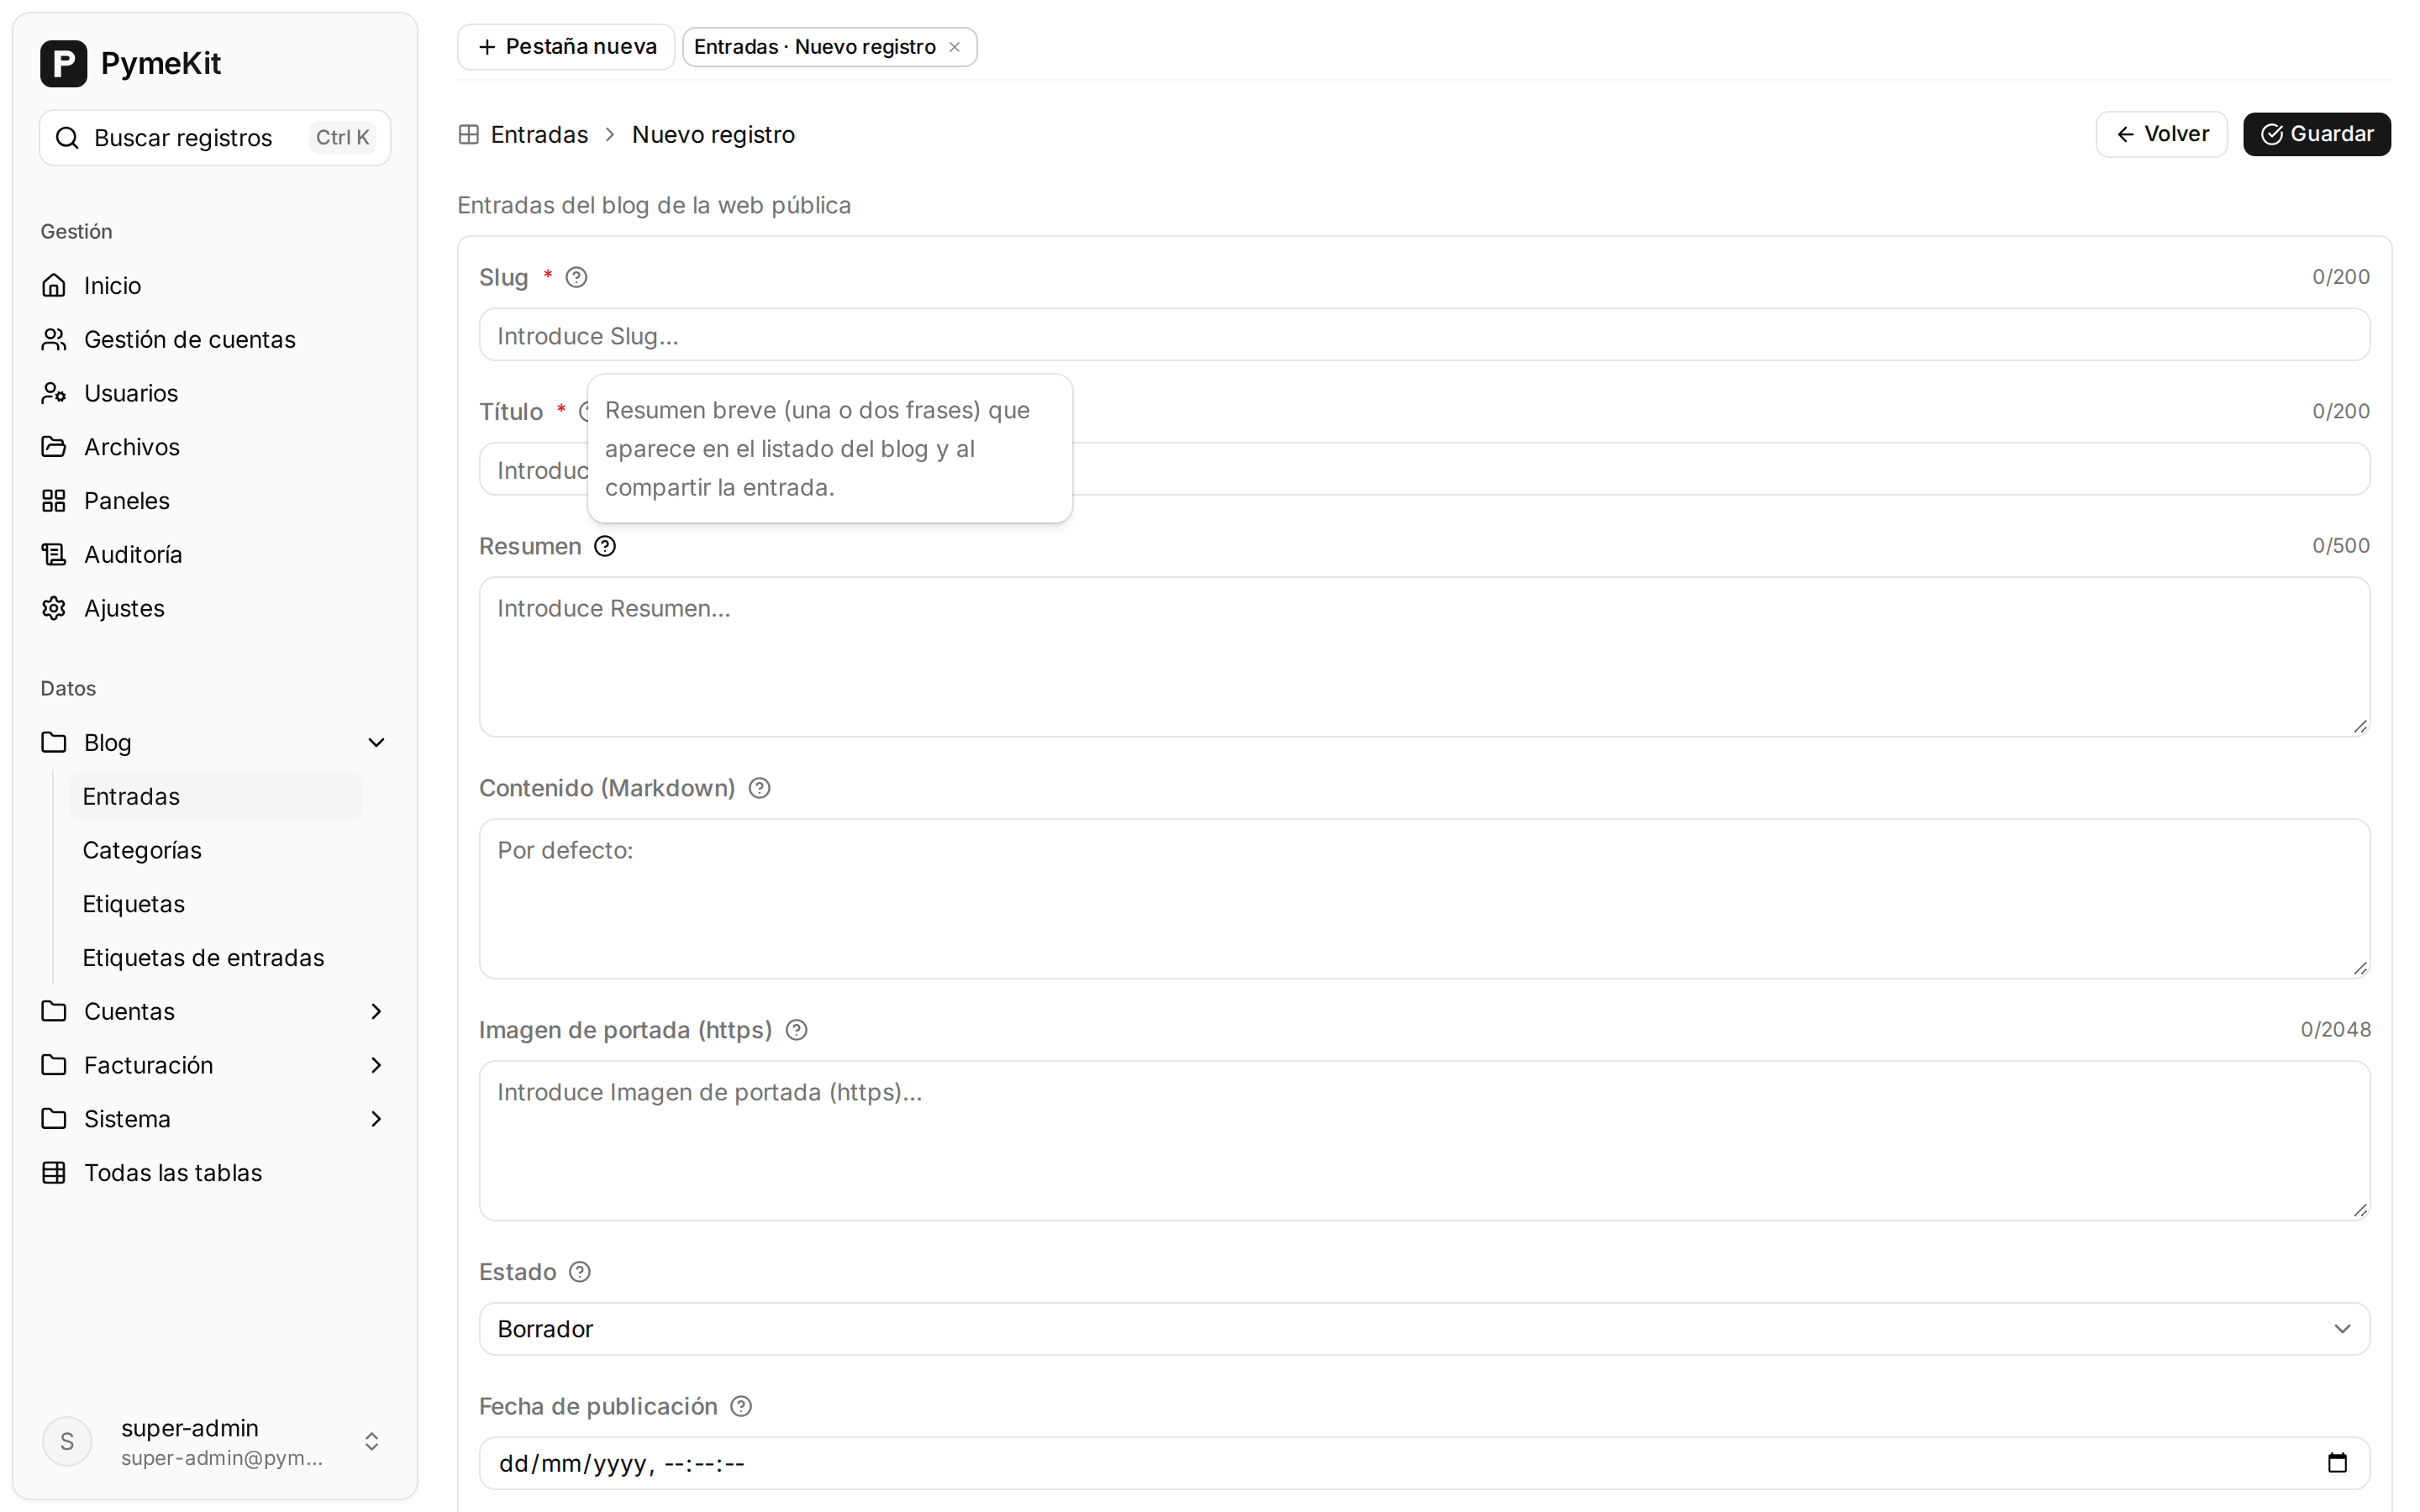
\includegraphics[width=0.92\textwidth]{figures/consola-ayuda.png}
    \caption{Formulario de alta de una entrada con la ayuda contextual «?» del
      campo «Resumen» abierta.}
    \label{fig:dis-consola-ayuda}
  \end{subfigure}
  \caption{Consola de administración de PymeKit (capturas de la aplicación).}
  \label{fig:dis-consola}
\end{figure}

\subsection{Ayuda contextual y resúmenes}
\label{sec:dis-ayudas}

Para que la consola la pueda usar personal no técnico, cada pantalla muestra
bajo el título un \textbf{resumen} de una o dos frases que explica para qué
sirve; en el explorador, ese resumen es la descripción de la tabla guardada en
sus metadatos. Además, cada campo de los formularios de la consola lleva una
\textbf{ayuda contextual «?»}, un componente reutilizable de la biblioteca de
interfaz que muestra al pulsarlo qué significa el campo y qué efecto tiene.
Ambos textos pasan por el sistema de traducción.

\subsection{Internacionalización}
\label{sec:dis-i18n}

La interfaz solo ofrece español (ADR-021): PymeKit se dirige a pymes
españolas y mantener dos idiomas duplicaría el coste de cada texto. Sin
embargo, se conserva toda la infraestructura de traducción: ningún texto
visible se escribe en el código ---tampoco atributos como \texttt{aria-label}
o \texttt{placeholder}---, sino que se referencia por clave a los mensajes del
idioma (\texttt{packages/i18n/src/messages/es}); la lista de idiomas está en
la configuración y una prueba unitaria comprueba la coherencia de las claves.
Añadir un idioma consiste en crear su carpeta de mensajes y registrarlo,
y se documenta como \emph{punto de extensión}. Los identificadores, las
tablas y las columnas siguen en inglés, como es habitual en el ecosistema
(ADR-003); sus nombres visibles en español son datos del CMS.

% ---------------------------------------------------------------------
\section{Decisiones de diseño principales}
\label{sec:dis-decisiones}

Cada decisión relevante se registró en el momento de tomarla con su contexto,
alternativas y consecuencias. La tabla~\ref{tab:dis-adr} las resume; las
decisiones no se borran, sino que se marcan como sustituidas cuando dejan de
valer.

\begin{longtable}{@{}l>{\raggedright\arraybackslash}p{4.3cm}>{\raggedright\arraybackslash}p{5.6cm}>{\raggedright\arraybackslash}p{2.4cm}@{}}
  \caption{Resumen de decisiones de diseño (ADR) y alternativas descartadas.}\label{tab:dis-adr}\\
  \toprule
  \textbf{ADR} & \textbf{Decisión} & \textbf{Alternativas descartadas (motivo)} & \textbf{Req.} \\
  \midrule
  \endfirsthead
  \toprule
  \textbf{ADR} & \textbf{Decisión} & \textbf{Alternativas descartadas (motivo)} & \textbf{Req.} \\
  \midrule
  \endhead
  \bottomrule
  \endfoot
  001 & Partir de componentes base con licencia
    & Desarrollo completo desde cero (inviable en plazo); otras bases abiertas (menos completas en multi-tenant y RLS); CMS genéricos con otra base de datos u otro \textit{backend} & RNF-01, 04 \\
  002 & Monorepo único y una sola base de datos & Dos repositorios con la misma base de datos (CI, despliegue y documentación duplicados) & RF-09, RNF-04 \\
  003 & Comentarios y documentación en español; identificadores en inglés & Todo en español (choca con el ecosistema); todo en inglés (dificulta la evaluación) & RF-13, RNF-05 \\
  004 & Un único CMS, de datos, sin CMS de contenidos basado en ficheros & Mantener dos CMS (complejidad sin aportar al objetivo) & RF-09 \\
  005 & Plataforma genérica sin dominio de negocio concreto & Implementar un dominio de ejemplo (desvía el esfuerzo de la base reutilizable) & RNF-01 \\
  006 & Flujo de desarrollo sin comprobaciones remotas de licencia & Mantenerla (dependencia de red y de un servicio externo) & --- \\
  007 & La memoria no nombra los componentes base & --- & --- \\
  008 & Descartar el servidor MCP y los generadores de código ligados a documentación externa & Conservarlos renombrados (dependen de documentación no incluida) & RNF-04 \\
  009 & La web escucha en el puerto 3100 & Puerto por defecto (ocupado en el equipo de desarrollo, B-02) & RNF-07 \\
  010 & Aislar de Internet los servicios locales & Confiar en el cortafuegos del sistema (los contenedores se lo saltan, B-04) & RNF-02 \\
  011 & CMS integrado: API Hono en \texttt{/api/cms}, pantallas como rutas de la web & Aplicaciones separadas (tres servicios, dos inicios de sesión); híbrida (dos enrutadores) & RF-08--11 \\
  012 & Esquema SQL del CMS llamado \texttt{cms} & Conservar el nombre original (excepción permanente en los controles automáticos) & RF-09 \\
  013 & Una sola pila de librerías en toda la web & Mantener las del CMS (dos formas de hacer lo mismo; dos sistemas de i18n) & RNF-05 \\
  014 & Super-administrador como raíz del CMS; RBAC del CMS para el resto del personal & Solo super-administrador, sin RBAC granular (incumple RF-09) & RF-08, 09 \\
  015 & Endurecer la seguridad del CMS & Aceptar el código sin auditar (brechas confirmadas, B-05--B-09) & RNF-02, 03 \\
  016 & Consola para super-administrador y personal del CMS, siempre con \texttt{aal2} & Dejar entrar con el \textit{claim} de acceso sin comprobar el AAL (B-14) & RF-08, RNF-02 \\
  017 & Blog en la base de datos gestionado desde el CMS & Blog fuera (debilita la gestión de contenidos); CMS de ficheros (dos CMS) & RF-01, 09 \\
  018 & Instantánea del autor en la auditoría & Claves ajenas \texttt{RESTRICT} (impide borrar usuarios); borrado lógico (más complejo) & RF-10 \\
  019 & Paneles con cuadrícula propia, sin librería & Librería de cuadrícula (más dependencias; arrastrar sin teclado no es accesible) & RF-11, RNF-08 \\
  020 & Consola por áreas de negocio, nombres en español como datos y sin esquema de demostración & Traducir nombres en el cliente; áreas fijas en un fichero; quitar equipos y pagos & RF-09, RNF-01, 08 \\
  021 & Interfaz solo en español conservando la infraestructura i18n & Mantener dos idiomas (doble mantenimiento); eliminar la i18n (impide traducir) & RF-13, RNF-01 \\
  022 & Una sola imagen Docker para la web y Supabase externa & Contenedores separados para la API del CMS; Supabase autoalojada en el mismo \textit{compose} & RNF-04, 07 \\
  023 & Comentarios didácticos en español limitados al núcleo de la arquitectura & Reescribir todos los comentarios (coste desproporcionado); no reescribir ninguno & RNF-05 \\
  024 & Rol intermedio «Encargado» en los equipos & Mantener solo propietario y miembro; dar al miembro más permisos & RF-06, RNF-01 \\
  025 & Planes de ejemplo para pymes en euros con ids de precio por variables & Ids fijos en el fichero; planes sin precios & RF-07, RNF-01 \\
  026 & Plantilla de roles del CMS en una migración de datos idempotente & Solo en el \textit{seed} (no llega a producción); roles de sistema no editables & RF-09, RNF-01 \\
  027 & Despliegue de referencia local con Docker, verificado desde cero; la nube queda documentada & Instancia pública en la nube (cuentas de pago y API de la base de datos expuesta, sin exigirlo la propuesta) & RNF-07 \\
\end{longtable}

% ---------------------------------------------------------------------
\section{Configuración reutilizable}
\label{sec:dis-configuracion}

La reutilización por configuración (RNF-01) se apoya en tres mecanismos, de
menor a mayor dinamismo.

\paragraph{Ficheros de configuración tipados.} Todo lo que cambia de un
producto a otro se concentra en \texttt{apps/web/src/config/*.config.ts}
(tabla~\ref{tab:dis-config}). Cada fichero valida su contenido con un esquema
Zod al arrancar, de modo que una configuración incorrecta falla pronto y con
un mensaje claro, en lugar de en tiempo de ejecución.

\begin{table}[htbp]
  \centering
  \footnotesize
  \caption{Ficheros de configuración de la aplicación.}
  \label{tab:dis-config}
  \begin{tabularx}{\textwidth}{@{}>{\raggedright\arraybackslash}p{4.4cm}X@{}}
    \toprule
    \textbf{Fichero} & \textbf{Qué configura} \\
    \midrule
    \texttt{app.config.ts} & Nombre del producto, título, descripción, URL y tema por defecto \\
    \texttt{auth.config.ts} & Métodos de acceso (contraseña, enlace mágico, OAuth) y captcha \\
    \texttt{account-mode.config.ts} & Modo de cuentas: personal, equipos o híbrido \\
    \texttt{feature-flags.config.ts} & Interruptores de funcionalidad derivados del modo y de las variables de entorno \\
    \texttt{billing.config.ts} & Proveedor de pago, productos, planes y precios \\
    \texttt{paths.config.ts} & Rutas de la aplicación \\
    \path{navigation.config.tsx}, \path{marketing-navigation.config.tsx} & Menús del área privada y de la web pública \\
    \texttt{tfg.config.ts} & Bloque académico de la página de inicio \\
    \bottomrule
  \end{tabularx}
\end{table}

\paragraph{Variables de entorno.} Los valores que dependen de la instalación
se leen de variables de entorno. Las públicas llevan el prefijo
\texttt{VITE\_} y los secretos (claves de la base de datos y de la pasarela)
nunca. Los interruptores de los módulos opcionales son:

\begin{itemize}
  \item \textbf{Equipos}: \path{VITE_ACCOUNT_MODE}
        (\texttt{personal-only}, \texttt{organizations-only} o
        \texttt{hybrid}) decide qué superficies de cuenta existen, y
        \path{VITE_ENABLE_TEAM_ACCOUNTS_CREATION} y
        \texttt{\ldots\_DELETION} las afinan. El modo es la única fuente de
        verdad: un interruptor granular nunca puede reactivar una superficie
        que el modo desactiva.
  \item \textbf{Facturación}: \path{VITE_BILLING_PROVIDER} y
        \path{VITE_ENABLE_PERSONAL_ACCOUNT_BILLING} /
        \path{VITE_ENABLE_TEAM_ACCOUNTS_BILLING}; la base de datos
        mantiene el mismo interruptor en su tabla de configuración para que
        las políticas RLS también lo respeten.
  \item \textbf{Bloque TFG}: \path{VITE_SHOW_TFG_INFO=false} deja la web
        limpia de cualquier referencia académica.
  \item \textbf{Otros}: notificaciones (y su modo en tiempo real), selector
        de tema, baja de cuentas y métodos de autenticación.
\end{itemize}

\paragraph{Configuración como datos.} Lo que la pyme debe poder cambiar sin
desplegar se guarda en la base de datos y se edita desde la consola: el
nombre visible, la descripción y el área de cada tabla, el formato de sus
columnas y el diseño de sus fichas (metadatos del CMS); los roles y permisos
del personal; y las preferencias globales, como la obligatoriedad del MFA.

Finalmente, el monorepo incluye generadores para crear paquetes nuevos con la
estructura y las dependencias correctas, de modo que la lógica propia de un
producto se añade como un paquete más sin modificar el núcleo. El
generador \texttt{package} (\texttt{pnpm turbo gen package}) pregunta si se
trata de una funcionalidad de negocio (\texttt{packages/features}) o de un
paquete de infraestructura y crea su \texttt{package.json},
\texttt{tsconfig.json} y punto de entrada, tomando las versiones del catálogo
del monorepo. Los generadores heredados para otras plataformas de despliegue
se retiraron porque producían configuración de otro \textit{framework}. Toda
esta configuración ---ficheros, variables de entorno, interruptores de
módulos, identidad visual, roles, planes y tablas propias en el CMS--- está
documentada en la guía \texttt{docs/CONFIGURACION.md} del repositorio.



\chapter{Construcción del Sistema}
% =====================================================================
% Capítulo: Construcción del Sistema
% Fuentes: docs/tfg/{PLAN,PROGRESO,BITACORA,DECISIONES,TRAZABILIDAD}.md,
% MAPA-REFERENCIAS.md (solo como guía; no se nombran las referencias),
% AGENTS.md, .claude/{settings.json,hooks,skills,agents},
% apps/web/supabase/{schemas,migrations}, packages/cms/*,
% packages/function-middleware, apps/web/src. Estado: F3c cerrada.
% =====================================================================

% Estilo de los extractos de código de este capítulo: letra pequeña, marco
% y sustitución de los caracteres acentuados (listings no admite UTF-8
% multibyte de forma nativa).
\lstdefinestyle{pymekit}{
  basicstyle=\ttfamily\scriptsize,
  breaklines=true,
  frame=single,
  columns=fullflexible,
  keepspaces=true,
  showstringspaces=false,
  numbers=left,
  numberstyle=\tiny,
  numbersep=6pt,
  xleftmargin=1.2em,
  literate={á}{{\'a}}1 {é}{{\'e}}1 {í}{{\'i}}1 {ó}{{\'o}}1 {ú}{{\'u}}1
           {Á}{{\'A}}1 {É}{{\'E}}1 {Í}{{\'I}}1 {Ó}{{\'O}}1 {Ú}{{\'U}}1
           {ñ}{{\~n}}1 {Ñ}{{\~N}}1 {ü}{{\"u}}1 {¿}{{?`}}1 {¡}{{!`}}1
           {«}{{\guillemotleft}}1 {»}{{\guillemotright}}1
}

Este capítulo describe cómo se ha construido PymeKit: el entorno y las
herramientas, la estructura del código, el punto de partida y las aportaciones
del trabajo, la secuencia de incrementos, una selección de extractos de
código representativos y los problemas más relevantes que se resolvieron.

% ---------------------------------------------------------------------
\section{Entorno y herramientas}
\label{sec:imp-entorno}

El desarrollo se ha realizado en un servidor Linux remoto, accedido por SSH,
con las herramientas de la tabla~\ref{tab:imp-herramientas}. La base de datos
local (PostgreSQL, autenticación y almacenamiento) se ejecuta en contenedores
con la CLI de Supabase; como el servidor tiene IP pública, sus puertos se
filtran explícitamente y la aplicación se consulta a través de un túnel SSH
(ADR-010).

\begin{table}[htbp]
  \centering
  \footnotesize
  \caption{Herramientas del entorno de desarrollo.}
  \label{tab:imp-herramientas}
  \begin{tabularx}{\textwidth}{@{}>{\raggedright\arraybackslash}p{3.4cm}X@{}}
    \toprule
    \textbf{Ámbito} & \textbf{Herramienta} \\
    \midrule
    Lenguaje y ejecución & TypeScript en modo estricto, Node.js (versión LTS) \\
    Monorepo & pnpm (con catálogo de versiones compartido) y Turborepo~\cite{turborepo} \\
    Aplicación & TanStack Start, Router y Query; React 19; Vite; Tailwind CSS 4 \\
    CMS & Hono, Drizzle ORM, Zod \\
    Base de datos & Supabase CLI (PostgreSQL, Auth, Storage) en contenedores Docker \\
    Pagos & Stripe en modo de pruebas y su CLI para reenviar \textit{webhooks} \\
    Pruebas & Vitest (unitarias), pgTAP~\cite{pgtap} (base de datos), Playwright~\cite{playwright} (E2E) \\
    Calidad & Oxlint y Oxfmt (análisis estático y formato), comprobación de tipos y de dependencias del monorepo \\
    Control de versiones & Git, GitHub (repositorio privado) y GitHub Actions; mensajes según Conventional Commits~\cite{conventionalcommits} \\
    Memoria & \LaTeX{} con la plantilla oficial de la escuela \\
    \bottomrule
  \end{tabularx}
\end{table}

La integración continua (\texttt{.github/workflows/ci.yml}) tiene tres
trabajos: \emph{Controles del TFG} (controles automáticos del repositorio, bloqueantes, e
informe de comentarios en inglés), \emph{TypeScript} (tipos, \textit{lint}, formato y
pruebas unitarias en cada \textit{push} a la rama principal y en cada \textit{pull request}) y
\emph{Supabase + E2E} (base de datos local, pgTAP, \textit{build} de pruebas y
Playwright), que por su coste solo se ejecuta en las \textit{pull requests}
hacia la rama principal o a mano.

% ---------------------------------------------------------------------
\section{Estructura del código}
\label{sec:imp-estructura}

La figura~\ref{fig:imp-arbol} muestra la estructura del repositorio. La
aplicación web es la única aplicación desplegable; todo lo demás son paquetes
que la componen o herramientas de verificación.

\begin{figure}[htbp]
  \centering
\begin{lstlisting}[style=pymekit, numbers=none, frame=none]
apps/
  web/                      TanStack Start + React 19 (una sola aplicación)
    src/routes/             rutas por fichero
      _marketing/           web pública: inicio, precios, blog, legales
      _authenticated/       área privada (sesión viva y MFA)
      admin/                consola: plataforma (super-admin) y cms/ (CMS)
      api/                  rutas de servidor: cms/$, billing/webhook, db/...
    src/lib/                server functions (*.functions.ts), servicios (*.server.ts)
    src/config/             configuración reutilizable (*.config.ts)
    supabase/               schemas/ (00-55), migrations/, tests/database (pgTAP)
  e2e/                      pruebas Playwright de la web y del CMS
packages/
  ui, i18n, shared, supabase, function-middleware, policies, otp, ...
  features/{auth,accounts,team-accounts,admin,notifications}
  billing/{core,gateway,stripe}
  cms/                      27 paquetes @pymekit/cms-*: api, auth, data-explorer,
                            filters, query-builder, audit-logs, dashboards, ...
                            y sus paquetes cliente *-ui
docs/tfg/                   plan, requisitos, decisiones, bitácora, trazabilidad
scripts/tfg/                controles automáticos del repositorio y etiquetas
memoria/                    esta memoria
\end{lstlisting}
  \caption{Estructura simplificada del repositorio.}
  \label{fig:imp-arbol}
\end{figure}

Las convenciones más importantes, recogidas en las directrices del
repositorio (\texttt{AGENTS.md}), son:

\begin{itemize}
  \item las \textit{server functions} se definen en ficheros
        \texttt{*.functions.ts} con la cadena
        \texttt{.middleware(\ldots).validator(Esquema).handler(\ldots)};
  \item los módulos solo de servidor llevan el sufijo \texttt{.server.ts} y
        un \textit{plugin} de Vite impide que lleguen al navegador;
  \item en el CMS, cada funcionalidad es un paquete con un servicio Drizzle
        (clase y fábrica \texttt{createXService()}), sus rutas Hono y
        funciones puras en \texttt{utils/};
  \item ningún texto visible se escribe en el código (todo pasa por i18n), y
        los registros usan el \textit{logger} compartido, nunca
        \texttt{console.log};
  \item los puntos clave se marcan con comentarios \texttt{[TFG] RF-xx} que
        un script recopila en la matriz de trazabilidad (275 etiquetas en su
        última generación).
\end{itemize}

% ---------------------------------------------------------------------
\section{Punto de partida y aportaciones}
\label{sec:imp-reutilizacion}

El desarrollo partió de componentes base con licencia comercial ---una base de
aplicación SaaS y un CMS para la base de datos--- (ADR-001). Sobre ellos, las
aportaciones de este trabajo son las que recoge la
tabla~\ref{tab:imp-reutilizacion}.

\begin{longtable}{@{}>{\raggedright\arraybackslash}p{4.2cm}>{\raggedright\arraybackslash}p{10.0cm}@{}}
  \caption{Aportaciones del trabajo.}\label{tab:imp-reutilizacion}\\
  \toprule
  \textbf{Aportación} & \textbf{Contenido} \\
  \midrule
  \endfirsthead
  \toprule
  \textbf{Aportación} & \textbf{Contenido} \\
  \midrule
  \endhead
  \bottomrule
  \endfoot
  Integración del CMS en la web & Montaje de la API en \texttt{/api/cms}, llamada en proceso durante el SSR y guardas de la consola (ADR-011, ADR-016); enlace entre el super-administrador y el rol raíz del CMS (ADR-014); pantallas del CMS como rutas de la web; esquema \texttt{cms} en la base de datos única (ADR-012) \\
  Unificación de la pila & Formularios, textos y componentes de interfaz del CMS sobre las mismas librerías que el resto de la web: unos 64 formularios y unos 183 ficheros con textos (ADR-013) \\
  Consola por áreas y ayudas & Consola organizada por áreas de negocio, nombres en español de las tablas como datos, ayuda contextual «?» y resúmenes en cada pantalla (ADR-020) \\
  Interfaz en español & Unas 1.770 claves, correos y plantillas en español sobre una infraestructura de internacionalización extensible (ADR-021) \\
  Blog & Blog en la base de datos gestionado desde el CMS, con lectura pública por RLS y rutas públicas (ADR-017) \\
  Auditoría & Registro de auditoría no falsificable, con instantánea del autor (ADR-018) \\
  Paneles & Cuadrícula propia de los paneles con \textit{widgets} de métrica, gráfica y tabla (ADR-019) \\
  Endurecimiento de seguridad & Revisiones adversariales de RLS y de seguridad; 29 fallos de seguridad corregidos y cubiertos por pruebas de regresión (ADR-015; capítulo de Pruebas); pruebas pgTAP de aislamiento \\
  Despliegue & Despliegue de la plataforma y su manual (ADR-022) \\
  Evaluación de la reutilización & Escenario de reutilización y medición de los cambios necesarios (anexo~\ref{cap:evaluacion}) \\
  Documentación & Plan, requisitos, decisiones, bitácora, trazabilidad, manuales de usuario y de desarrollador, comentarios didácticos en español y bloque académico configurable \\
\end{longtable}

% ---------------------------------------------------------------------
\section{Construcción por incrementos}
\label{sec:imp-fases}

El sistema se ha construido en incrementos, cada uno funcional y verificado
antes de pasar al siguiente, con su rama de trabajo y su
\textit{pull request}. La tabla~\ref{tab:imp-fases} resume el contenido de
cada incremento y el estado de las pruebas a su cierre; la planificación
temporal se presenta en el capítulo de Planificación.

\begin{longtable}{@{}l>{\raggedright\arraybackslash}p{9.6cm}>{\raggedright\arraybackslash}p{3.0cm}@{}}
  \caption{Incrementos de construcción y estado de las pruebas al cerrarlos.}\label{tab:imp-fases}\\
  \toprule
  \textbf{Fase} & \textbf{Contenido} & \textbf{Pruebas al cierre} \\
  \midrule
  \endfirsthead
  \toprule
  \textbf{Fase} & \textbf{Contenido} & \textbf{Pruebas al cierre} \\
  \midrule
  \endhead
  \bottomrule
  \endfoot
  F0 & Directrices de desarrollo, plan, requisitos, guías, controles automáticos del repositorio e integración continua mínima & --- \\
  F1 & Base de la aplicación web: renombrado del ámbito de paquetes a \texttt{@pymekit/*}, retirada de módulos no necesarios, base de datos local, puerto propio, CI completa & 61 unit.; pgTAP 27/396; E2E 43 \\
  F2.1 & Base de datos del CMS: esquema \texttt{cms}, pegamento super-administrador $\rightarrow$ Root, MFA obligatorio; primera revisión adversarial de RLS y corrección de dos brechas & pgTAP 57/1.550 \\
  F2.2 & API del CMS: 19 paquetes de servidor, Hono en \texttt{/api/cms}, autenticación con la sesión de la web & 1.130 unit.; 11 E2E de la API \\
  F2.3 & Base de la interfaz: consola compartida, guardas con \texttt{aal2}, cliente RPC, \textit{fetch} isomorfo & E2E 60 \\
  F2.4 & Explorador de datos: listado con filtros, orden, búsqueda, columnas y vistas; ficha con relaciones; creación, edición y borrado & 1.313 unit.; E2E 86 \\
  F2.5 & Exploradores de usuarios y de almacenamiento & E2E 102 \\
  F2.6 & Auditoría y búsqueda global; auditoría no falsificable y redactada según permisos & pgTAP 60/1.652; E2E 108 \\
  F2.6b & Blog en la base de datos gestionado desde el CMS y rutas públicas; formatos legibles & pgTAP 62/1.730; E2E 129 \\
  F2.7 & Ajustes: general, autenticación, miembros, RBAC (roles, grupos y permisos), recursos y diseñador de fichas & pgTAP 67/2.049; E2E 141 \\
  F2.8 & Paneles con \textit{widgets} de métrica, gráfica y tabla & pgTAP 2.060 \\
  F2.9 & Cierre de la integración del CMS: suite E2E completa & E2E 149 \\
  F3a--b & Español por defecto (unas 1.770 claves), correos y plantillas en español, identidad visual, etiquetas legibles de enumerados, sesión caducada & E2E 150 \\
  F3c & Consola por áreas de negocio, nombres en español de las tablas, retirada del esquema de demostración (ADR-020); solo español (ADR-021); ayuda «?» y resúmenes; bloque académico en la página de inicio & 1.691 unit.; pgTAP 70/2.073; E2E 156 \\
  F4 & Comentarios didácticos en español en el núcleo de la arquitectura: esquemas SQL, \textit{middleware} de autorización, clientes de base de datos, motor de políticas y \textit{server functions} (ADR-023) & --- \\
  F5 & Rol intermedio «Encargado» en los equipos (ADR-024), planes de ejemplo para pymes en euros (ADR-025), plantilla de roles del CMS (ADR-026), guía de configuración y generador de paquetes & pgTAP 72/2.098 \\
  F6 & Evaluación de la reutilización en un caso de estudio (anexo~\ref{cap:evaluacion}); auditoría automática de accesibilidad y medición del rendimiento con 10.000 cuentas, con sus correcciones (B-59, B-60); pago verificado con la pasarela en modo de pruebas, E2E de permisos de facturación y suplantación reactivada (B-61, B-62) & pgTAP 73/2.099; E2E con facturación \\
  F7 & Imagen de contenedor, orquestación y manual de instalación probado desde un clon limpio (ADR-022, ADR-027) & E2E 167 contra la imagen \\
\end{longtable}

Las cifras de pgTAP se expresan como ficheros/pruebas.

% ---------------------------------------------------------------------
\section{Extractos de código significativos}
\label{sec:imp-extractos}

Se presentan cinco extractos breves que ilustran las decisiones del capítulo
de Diseño. Se han recortado los comentarios y las líneas no esenciales.

\subsection{Una política RLS condicionada al permiso}

El extracto~\ref{lst:imp-rls} muestra la política que permite borrar una
invitación. No basta con pertenecer a la cuenta: hace falta además el permiso
\texttt{invites.manage} en ella. La llamada a \texttt{auth.uid()} va dentro de
\texttt{(select \ldots)} para que PostgreSQL la evalúe una sola vez por
consulta y no por cada fila.

\begin{lstlisting}[style=pymekit, language=SQL, caption={Política de borrado de invitaciones (\texttt{07-invitations.sql}).}, label={lst:imp-rls}]
create policy invitations_delete on public.invitations
  for delete to authenticated
  using (
    has_role_on_account (account_id)
    and public.has_permission (
      (select auth.uid ()),
      account_id,
      'invites.manage'::public.app_permissions
    )
  );
\end{lstlisting}

El blog (extracto~\ref{lst:imp-blog}) combina tres mecanismos: se revocan
todos los privilegios, se concede la lectura \emph{por columnas} (la web no
necesita saber qué usuario creó una entrada) y la política solo devuelve lo
publicado. La escritura no se concede a ningún rol de la API: se hace desde
el CMS, con sus funciones que comprueban el permiso.

\begin{lstlisting}[style=pymekit, language=SQL, caption={Lectura pública del blog (\texttt{19-blog.sql}, recortado).}, label={lst:imp-blog}]
alter table public.blog_posts enable row level security;
revoke all on public.blog_posts from anon, authenticated, service_role;
grant select, insert, update, delete on table public.blog_posts to service_role;

grant select (id, slug, title, excerpt, content, status,
              published_at, category_id /* ... */)
  on table public.blog_posts to anon, authenticated;

create policy blog_posts_read_published on public.blog_posts
  for select to anon, authenticated
  using (status = 'published' and published_at <= now());
\end{lstlisting}

\subsection{Una \textit{server function} protegida por \textit{middleware}}

El extracto~\ref{lst:imp-sfn} es la función que crea una sesión de pago para
un equipo; es la que materializa la segunda barrera del caso CU-04. La cadena
de \textit{middleware} gestiona los errores, exige sesión y comprueba el
permiso \texttt{billing.manage} sobre la cuenta indicada (consultando
\texttt{has\_permission} en la base de datos) antes de ejecutar el
manejador. Los datos de entrada se validan con un esquema Zod.

\begin{lstlisting}[style=pymekit, caption={Server function de pago de equipo (\texttt{billing.functions.ts}, recortado).}, label={lst:imp-sfn}]
const billingManageMiddleware = [
  errorMiddleware,
  authMiddleware,
  withFeaturePermission('billing.manage'),
];

export const createTeamAccountCheckoutSession = createServerFn({
  method: 'POST',
})
  .middleware(billingManageMiddleware)
  .validator(TeamCheckoutSchema)
  .handler(async ({ data }) => {
    if (!featureFlagsConfig.enableTeamAccountBilling) {
      throw new Error('Team account billing is not enabled');
    }

    const client = getSupabaseServerClient(); // cliente con RLS
    const service = createTeamBillingService(client);

    return service.createCheckout(data);
  });
\end{lstlisting}

\subsection{Montaje de la API del CMS y una ruta Hono}

La integración del CMS en la web (ADR-011) se reduce a una ruta de servidor
que reenvía cualquier petición bajo \texttt{/api/cms/} a la aplicación Hono
(extracto~\ref{lst:imp-montaje}). La importación dinámica dentro del
manejador garantiza que el código del CMS ---con el controlador de PostgreSQL
y la clave secreta--- nunca forme parte de un fragmento del navegador.

\begin{lstlisting}[style=pymekit, caption={Montaje de la API del CMS (\texttt{routes/api/cms/\$.ts}).}, label={lst:imp-montaje}]
async function handleCmsApiRequest({ request }: { request: Request }) {
  const { getCmsApiApp } = await import('#/lib/cms/cms-api-app.server.ts');
  const app = await getCmsApiApp();

  return app.fetch(request);
}

export const Route = createFileRoute('/api/cms/$')({
  server: {
    handlers: {
      GET: handleCmsApiRequest,
      POST: handleCmsApiRequest,
      // ... PUT, PATCH, DELETE y OPTIONS igual
    },
  },
});
\end{lstlisting}

Cada funcionalidad del CMS registra sus rutas en la aplicación Hono
(extracto~\ref{lst:imp-hono}): valida la entrada, delega la autorización y la
consulta en su servicio y traduce cualquier error a un código estable, sin
exponer el mensaje interno.

\begin{lstlisting}[style=pymekit, caption={Ruta del registro de auditoría (\texttt{get-audit-logs-route.ts}, recortado).}, label={lst:imp-hono}]
export function registerAuditLogsRoute(router: Hono) {
  return router.get(
    '/v1/audit-logs',
    zValidator('query', AuditLogsQuerySchema, invalidAuditLogsInput),
    async (c) => {
      const { cursor, limit, ...filters } = c.req.valid('query');

      try {
        const data = await createAuditLogsService(c).getAuditLogs({
          cursor, limit, filters,
        });
        return c.json(data);
      } catch (error) {
        // 4xx/5xx con código estable (AUDIT_LOG_*); el detalle va al log
        return respondWithAuditLogsError(c, error, { route: 'list' });
      }
    },
  );
}
\end{lstlisting}

El servicio ejecuta cada consulta dentro de una transacción en la que antes
fija la identidad del usuario (extracto~\ref{lst:imp-claims}). Los valores se
pasan como \emph{parámetros enlazados}, nunca concatenados en el texto SQL, y
el rol se limita a los que puede llevar un JWT de usuario. Así, las políticas
RLS del esquema \texttt{cms} se aplican a la API igual que a cualquier otro
cliente.

\begin{lstlisting}[style=pymekit, caption={Identidad del usuario en cada transacción del CMS (\texttt{drizzle-client.ts}, recortado).}, label={lst:imp-claims}]
const role = ALLOWED_DB_ROLES.has(token.role) ? token.role : 'anon';
const claims = JSON.stringify(token);

return rlsClient.transaction(async (tx) => {
  await tx.execute(sql`select set_config('request.jwt.claims', ${claims}, true)`);
  await tx.execute(sql`select set_config('request.jwt.claim.sub', ${sub}, true)`);
  await tx.execute(sql`select set_config('role', ${role}, true)`);

  return await transaction(tx);
});
\end{lstlisting}

\subsection{La migración de las áreas de la consola}

La consola por áreas (ADR-020) no necesitó cambios de estructura: el área de
cada tabla se guarda en el campo \texttt{ui\_config} de sus metadatos, que ya
existía. La migración (extracto~\ref{lst:imp-areas}) carga los valores por
defecto en una tabla temporal y los aplica \emph{solo} donde no hay un valor
propio, de modo que nunca pisa lo que una pyme haya personalizado desde
Ajustes $\rightarrow$ Recursos y puede ejecutarse de nuevo sin efectos.

\begin{lstlisting}[style=pymekit, language=SQL, caption={Áreas de navegación del CMS (\texttt{20261002140000\_cms\_navigation\_groups.sql}, recortado).}, label={lst:imp-areas}]
insert into cms_navigation_defaults
    (schema_name, table_name, navigation_group, display_name, previous_names, ordering)
values
    ('public', 'blog_posts', 'Blog', 'Entradas', array['Blog: entradas'], 100),
    ('public', 'accounts', 'Cuentas', 'Cuentas', array['Cuentas'], 200),
    ('public', 'subscriptions', 'Facturación', 'Suscripciones',
     array['Facturación: suscripciones'], 310),
    ('public', 'config', 'Sistema', 'Configuración',
     array['Configuración de la plataforma'], 400);
    -- ... resto de tablas

-- Área: solo si la tabla todavía no tiene una.
update cms.table_metadata as meta
set ui_config = coalesce(meta.ui_config, '{}'::jsonb)
        || jsonb_build_object('navigation_group', defaults.navigation_group)
from cms_navigation_defaults as defaults
where meta.schema_name = defaults.schema_name
  and meta.table_name = defaults.table_name
  and nullif(btrim(meta.ui_config ->> 'navigation_group'), '') is null;
\end{lstlisting}

% ---------------------------------------------------------------------
\section{Problemas relevantes resueltos}
\label{sec:imp-problemas}

Todas las incidencias se registraron en una bitácora en el momento de
producirse, con el formato «qué pasó, causa, solución, evidencia y lección».
Hasta la fecha de corte se registraron 60. La tabla~\ref{tab:imp-bitacora} recoge
una selección de las no relacionadas directamente con el control de acceso;
las de seguridad se analizan en el capítulo de Pruebas
(sección~\ref{sec:pru-seguridad}).

\begin{longtable}{@{}l>{\raggedright\arraybackslash}p{4.8cm}>{\raggedright\arraybackslash}p{7.4cm}@{}}
  \caption{Selección de problemas resueltos y lecciones aprendidas (bitácora del proyecto).}\label{tab:imp-bitacora}\\
  \toprule
  \textbf{ID} & \textbf{Problema} & \textbf{Solución y lección} \\
  \midrule
  \endfirsthead
  \toprule
  \textbf{ID} & \textbf{Problema} & \textbf{Solución y lección} \\
  \midrule
  \endhead
  \bottomrule
  \endfoot
  B-01 & El renombrado masivo del ámbito de paquetes no alcanzó una expresión regular donde aparecía escapado & Se corrigió y los controles automáticos detectan ahora también las variantes escapadas. Un renombrado masivo se verifica buscando variantes, no solo la forma literal. \\
  B-04 & La base de datos local quedó accesible desde Internet porque los contenedores se saltan el cortafuegos & Regla de filtrado específica para contenedores y acceso por túnel SSH (ADR-010). En un servidor con IP pública, «local» no significa privado. \\
  B-10 & Esquema declarativo y migraciones del CMS desincronizados (nueve funciones distintas) & Se alinearon con las migraciones. La comparación de esquemas forma parte de la verificación de cualquier cambio de base de datos. \\
  B-11 & Una prueba existente se titulaba «MFA obligatorio por defecto», pero su aserción comprobaba que se concedía el acceso & Se reescribió. Una prueba en verde solo demuestra que el sistema hace lo que dice la prueba: hay que leer las aserciones. \\
  B-16 & Ciclo de dependencias al poner componentes y API del explorador en el mismo paquete & Paquete cliente separado. Separar cliente y servidor también evita ciclos. \\
  B-17, B-29 & La API respondía 500 a registros inexistentes porque el envoltorio de errores perdía el código de PostgreSQL & Se conserva la causa y se traduce el código SQLSTATE a 403/404. Sin la causa no se distingue «no existe» de «ha fallado». \\
  B-35 & La herramienta de comparación de esquemas omitía la opción \texttt{security\_invoker} de una vista y los permisos por columna & Esa parte de la migración se escribe a mano y pgTAP comprueba ambas propiedades. Que la comparación salga limpia no demuestra que la migración sea segura. \\
  B-36 & La sincronización de tablas del CMS duplicaba las relaciones en cada ejecución & Función idempotente, cubierta por pgTAP. \\
  B-52 & Tras cambiar de rama, el servidor de desarrollo conservaba un árbol de rutas sin el CMS & Reinicio limpiando cachés. Que las pruebas pasen contra la \textit{build} no garantiza que el entorno de desarrollo esté sano. \\
  B-53 & Una sesión revocada pero con firma válida rompía la consola & Comprobación con estado de la sesión en la entrada de las rutas protegidas. Verificar la firma de un JWT no demuestra que la sesión exista. \\
  B-55 & La lista de miembros superaba el tiempo máximo con unos cientos de cuentas (función volátil evaluada por fila) & Envolver la llamada en \texttt{(select \ldots)}; véase la sección~\ref{sec:pru-rendimiento}. \\
\end{longtable}



\chapter{Pruebas del Sistema}
% =====================================================================
% Capítulo: Pruebas del Sistema
% Fuentes: apps/web/supabase/tests/database (pgTAP), *.test.ts(x) (Vitest),
% apps/e2e/tests (Playwright), .github/workflows/ci.yml,
% docs/tfg/{PROGRESO,BITACORA,TRAZABILIDAD,DECISIONES}.md,
% .claude/skills/rls-review. Cifras: recuento de ficheros con grep y última
% verificación registrada (F3c); unitarias confirmadas con `pnpm test:unit`.
% =====================================================================

% Estilo de los extractos de este capítulo (mismo criterio que en
% Construcción: listings no admite UTF-8 multibyte de forma nativa).
\lstdefinestyle{pymekitpru}{
  basicstyle=\ttfamily\scriptsize,
  breaklines=true,
  frame=single,
  columns=fullflexible,
  keepspaces=true,
  showstringspaces=false,
  literate={á}{{\'a}}1 {é}{{\'e}}1 {í}{{\'i}}1 {ó}{{\'o}}1 {ú}{{\'u}}1
           {ñ}{{\~n}}1 {Á}{{\'A}}1 {É}{{\'E}}1 {Ó}{{\'O}}1 {Ú}{{\'U}}1
}

Este capítulo presenta la estrategia de pruebas de PymeKit y sus
resultados: pruebas unitarias, de integración con la base de datos y la API
del CMS, pruebas de sistema funcionales (E2E por caso de uso) y no
funcionales (seguridad y rendimiento), y pruebas de aceptación. Termina con
las cifras globales y la matriz de trazabilidad entre requisitos y pruebas.

% ---------------------------------------------------------------------
\section{Estrategia de pruebas}
\label{sec:pru-estrategia}

La estrategia sigue el criterio de la pirámide de pruebas: muchas pruebas
rápidas y aisladas en la base, y pocas pruebas de extremo a extremo en la
cima. Su rasgo distintivo es que la base de datos tiene su propio nivel de
pruebas, porque en PymeKit es la frontera de autorización (sección~\ref{sec:dis-seguridad}):
una política RLS mal escrita no se detecta con pruebas de la interfaz, ya que
la interfaz no ofrece el camino para explotarla.

\begin{table}[htbp]
  \centering
  \footnotesize
  \caption{Niveles de prueba, herramientas y qué verifica cada uno.}
  \label{tab:pru-niveles}
  \begin{tabularx}{\textwidth}{@{}>{\raggedright\arraybackslash}p{2.6cm}>{\raggedright\arraybackslash}p{2.4cm}X@{}}
    \toprule
    \textbf{Nivel} & \textbf{Herramienta} & \textbf{Qué verifica} \\
    \midrule
    Unitarias & Vitest & Funciones puras y componentes: filtros, constructor de consultas, formateadores, cálculo de la cuadrícula de paneles, clasificación de errores, componentes de interfaz, coherencia de las claves de traducción \\
    Integración (base de datos) & pgTAP~\cite{pgtap} & Políticas RLS, privilegios, funciones y \textit{triggers}, ejecutados como usuarios reales; aislamiento entre cuentas y entre niveles de personal del CMS \\
    Integración (API del CMS) & Playwright (peticiones HTTP) & Autenticación, permisos y códigos de error de la API montada en la web \\
    Sistema (funcionales) & Playwright~\cite{playwright} & Casos de uso completos en el navegador contra la \textit{build} de pruebas \\
    Sistema (no funcionales) & pgTAP, revisión adversarial, revisión manual & Seguridad (intentos de ataque), rendimiento y usabilidad \\
    Aceptación & Revisión del autor y del tutor & Adecuación a la propuesta \\
    \bottomrule
  \end{tabularx}
\end{table}

Todas las pruebas automáticas forman parte de la integración continua
(sección~\ref{sec:imp-entorno}): las unitarias se ejecutan en cada
\textit{push} a la rama principal y en cada \textit{pull request}; pgTAP y E2E, solo en cada \textit{pull request} hacia la rama
principal. Además, cada cambio se cierra con una lista de verificación
obligatoria (tipos, \textit{lint}, formato, controles automáticos del repositorio, pruebas
afectadas, revisión adversarial del \textit{diff} y, si toca la base de
datos, revisión de RLS). Las pruebas E2E se ejecutan siempre contra la
\textit{build} de pruebas y no contra el servidor de desarrollo (B-13).

% ---------------------------------------------------------------------
\section{Pruebas unitarias}
\label{sec:pru-unitarias}

Hay 116 ficheros de pruebas unitarias repartidos en 28 paquetes, con 1.691
pruebas superadas y una omitida. La mayor parte corresponde a los paquetes
del CMS, que concentran la lógica algorítmica: paneles (262 pruebas), núcleo
del explorador de datos (234), constructor de consultas (222), formateadores
(218), núcleo de filtros (181) y componentes del explorador (137).

Algunas pruebas unitarias son, en realidad, pruebas de seguridad. Por
ejemplo, la de \texttt{buildParameterizedStatement} reproduce el valor
malicioso que permitía la inyección SQL de la incidencia B-24
(un nombre que contenía la cadena \texttt{\$2}) y comprueba que ahora viaja
como parámetro enlazado; y las de protección de usuarios verifican que nadie
puede actuar sobre sí mismo ni sobre un super-administrador (B-21). Otras
garantizan propiedades transversales, como que todas las claves de traducción
usadas existen en los mensajes en español.

% ---------------------------------------------------------------------
\section{Pruebas de integración}
\label{sec:pru-integracion}

\subsection{Base de datos: RLS y aislamiento multi-tenant}
\label{sec:pru-pgtap}

La batería pgTAP tiene 73 ficheros (71 de pruebas y 2 de utilidades) con
2.099 pruebas. Cada fichero se ejecuta dentro de una transacción que se
deshace al terminar; crea usuarios de prueba, se \emph{autentica} como cada
uno de ellos (fijando su JWT y el rol \texttt{authenticated} en la sesión,
como hace el servicio de autenticación) y comprueba qué puede ver y hacer.
Se organizan en cuatro grupos:

\begin{itemize}
  \item \textbf{Aislamiento de la plataforma} (cuentas personales y de
        equipo, membresías, invitaciones y sus límites, transferencia de
        propiedad, facturación, notificaciones, almacenamiento,
        super-administrador): un usuario solo ve y modifica lo de sus
        cuentas, y solo con el permiso adecuado.
  \item \textbf{Superficie de privilegios}: \texttt{privileges.test.sql}
        comprueba que ningún rol de la API conserva privilegios residuales
        (como \texttt{TRUNCATE}, que ignora RLS) y \texttt{anon-surface.test.sql}
        fija la superficie exacta del rol anónimo ---solo puede leer el blog
        y no ejecuta ninguna función--- y falla si se amplía (B-39).
  \item \textbf{Control de acceso del CMS} (41 ficheros): permisos de datos,
        sistema y almacenamiento, rangos, delegación, denegaciones,
        auditoría, paneles, vistas guardadas, búsqueda global y el pegamento
        con el super-administrador.
  \item \textbf{Regresión de seguridad}: un fichero por revisión adversarial
        (\texttt{cms-isolation}, \texttt{cms-audit-isolation},
        \texttt{cms-members-isolation}, \texttt{cms-rbac-isolation}\ldots) que
        conserva como prueba cada ataque estudiado.
\end{itemize}

El extracto~\ref{lst:pru-tenant} muestra el patrón básico de una prueba de
aislamiento: tras crear una suscripción para una cuenta, un usuario ajeno no
obtiene ninguna fila.

\begin{lstlisting}[style=pymekitpru, language=SQL, caption={Aislamiento de la facturación entre cuentas (\texttt{team-billing-subscriptions.test.sql}, recortado).}, label={lst:pru-tenant}]
select tests.create_supabase_user('foreigner');
select pymekit.authenticate_as('foreigner');

select is_empty(
  $$ select 1 from subscriptions where id = 'sub_test' $$,
  'The account cannot read the other account subscriptions'
);
\end{lstlisting}

Las pruebas de regresión de las revisiones adversariales ejecutan el ataque
tal como se descubrió. El extracto~\ref{lst:pru-ataque} reproduce la escalada
de la incidencia B-05: antes de la corrección la sentencia afectaba a una
fila; ahora debe fallar con el código de permiso denegado (\texttt{42501}).
La misma prueba comprueba a continuación que la operación legítima sigue
funcionando, para que la corrección no sea simplemente «bloquearlo todo».

\begin{lstlisting}[style=pymekitpru, language=SQL, caption={Regresión de la escalada por \texttt{UPDATE} sin \texttt{WITH CHECK} (\texttt{cms-isolation.test.sql}).}, label={lst:pru-ataque}]
select cms_tests.authenticate_as('iso_mid');

-- El ataque que funcionaba antes de la corrección (UPDATE 1)
select throws_ok(
    $$ update cms.role_permissions
       set permission_id = cms_tests.test_uuid(9304)
       where role_id = cms_tests.test_uuid(9202)
         and permission_id = cms_tests.test_uuid(9303) $$,
    '42501',
    null,
    'E1: no puede colgar de un rol inferior un permiso que no posee'
);
\end{lstlisting}

\subsection{API del CMS}
\label{sec:pru-api}

La API del CMS se prueba de dos formas. Sus servicios y utilidades tienen
pruebas unitarias con el cliente de datos simulado. Y la API montada en la
web se prueba con peticiones HTTP reales desde Playwright
(\texttt{cms-api.spec.ts} y las comprobaciones de API de los demás ficheros
del CMS): sin sesión responde 401; con sesión pero sin acceso al CMS, o sin
segundo factor, o con la cuenta del CMS desactivada, 403; una petición con
campos no permitidos (por ejemplo, metadatos de la aplicación al crear un
usuario) se rechaza con 400; y cada rechazo se comprueba por su código de
error estable, no solo por el estado HTTP, porque un 403 no demuestra nada si
no se sabe por qué se produjo (B-26).

% ---------------------------------------------------------------------
\section{Pruebas de sistema}
\label{sec:pru-sistema}

\subsection{Pruebas funcionales por caso de uso}
\label{sec:pru-funcionales}

Las pruebas E2E se organizan en 35 ficheros, 19 de ellos del CMS; la última
ejecución completa, con las de facturación, ejecutó 189 pruebas. Se ejecutan en español, el único idioma
de la interfaz, y un fichero específico comprueba que no queda ningún texto
en inglés visible. La tabla~\ref{tab:pru-cu} relaciona cada caso de uso con
las pruebas que lo cubren.

\begin{table}[htbp]
  \centering
  \footnotesize
  \caption{Cobertura E2E de los casos de uso.}
  \label{tab:pru-cu}
  \begin{tabularx}{\textwidth}{@{}l>{\raggedright\arraybackslash}p{5.0cm}>{\raggedright\arraybackslash}X@{}}
    \toprule
    \textbf{CU} & \textbf{Ficheros de prueba} & \textbf{Estado} \\
    \midrule
    CU-01 & \texttt{authentication/*} (registro, acceso, recuperación de contraseña, redirecciones, sesión caducada), \texttt{account} & Cubierto \\
    CU-02 & \texttt{team-accounts/*}, \texttt{invitations} (incluida la aceptación con MFA) & Cubierto, incluida la promoción a «Encargado» \\
    CU-03 & \texttt{team-billing}, \texttt{user-billing} (pago con la tarjeta de prueba y suscripción activa tras el aviso de la pasarela) & Cubierto con la cuenta de pruebas de Stripe \\
    CU-04 & \texttt{billing-permissions} (aviso en la interfaz y petición de pago rechazada por el servidor); pgTAP de facturación (base de datos) & Cubierto en las tres capas \\
    CU-05 & \texttt{admin} (404 sin permiso, MFA obligatorio, bloquear, reactivar, borrar, suplantar) & Cubierto; la suplantación se reactivó tras corregir B-61 \\
    CU-06 & \texttt{cms-data-explorer*}, \texttt{cms-audit-logs}, \texttt{cms-settings-*}, \texttt{cms-ui}, \texttt{cms-sidebar-areas}, \texttt{cms-field-help}, \texttt{cms-page-summaries} & Cubierto \\
    CU-07 & --- (caso de estudio, anexo~\ref{cap:evaluacion}) & Evaluado \\
    CU-08 & \texttt{blog} (lectura anónima, borradores invisibles, Markdown seguro, publicación desde el CMS, \textit{sitemap}) & Cubierto \\
    \bottomrule
  \end{tabularx}
\end{table}

Las pruebas del CMS verifican sistemáticamente los dos lados de cada
permiso: el personal de soporte, con un rol limitado, \emph{no} ve en la
barra lateral ni puede abrir por URL las tablas sin permiso, y el
super-administrador sí. Muchas incluyen además pruebas negativas
específicas derivadas de incidencias: la guarda de clave en la edición
(B-19), un HTML disfrazado de imagen en la subida de ficheros (B-25), el
\textit{widget} de una tabla no legible («sin acceso», B-50) o la consola con
una sesión sin segundo factor (B-14).

\subsection{Pruebas no funcionales: seguridad}
\label{sec:pru-seguridad}

La seguridad se ha verificado con revisiones adversariales en dos niveles:
una revisión del \textit{diff} orientada a la búsqueda de fallos al terminar
cada funcionalidad, y una revisión específica de RLS en cada cambio relevante
de políticas, privilegios o funciones de privilegios elevados.

La revisión de RLS parte de que leer las políticas no basta: hay que
\emph{demostrar} el aislamiento. Tras un inventario y una auditoría estática
con un catálogo de ataques, cada hallazgo plausible se convierte en una
prueba pgTAP que ejecuta el ataque como el usuario atacante y comprueba que
falla. Después, una revisión independiente, que solo recibe la política, la
prueba y la afirmación, intenta \emph{refutarla}: una brecha solo se acepta
si esa segunda revisión la reproduce, y un aprobado, solo si no encuentra un
vector abierto. La tabla~\ref{tab:pru-rls} resume las revisiones de RLS
realizadas.

\begin{table}[htbp]
  \centering
  \footnotesize
  \caption{Revisiones adversariales de RLS y su resultado.}
  \label{tab:pru-rls}
  \begin{tabularx}{\textwidth}{@{}l>{\raggedright\arraybackslash}p{3.4cm}X@{}}
    \toprule
    \textbf{Fase} & \textbf{Alcance} & \textbf{Resultado} \\
    \midrule
    F2.1 & Esquema \texttt{cms} completo tras su incorporación & Dos brechas confirmadas (B-05, B-08), cinco endurecimientos y cuatro funciones desalineadas (ADR-015). La refutación independiente encontró B-08 \\
    F2.6 & Auditoría y búsqueda global & Aislado; cuatro debilidades menores endurecidas (B-31 a B-34); +31 pruebas \\
    F2.6b & Blog y apertura del esquema \texttt{public} al rol anónimo & Aislado; riesgo latente de privilegios por defecto documentado y vigilado por prueba (B-39) \\
    F2.7a & Miembros del CMS y autor de la auditoría & Aislado; +68 pruebas; una inyección SQL latente (B-45) \\
    F2.7b & RBAC del CMS con administradores delegados de distintos rangos & Brecha de escape de denegaciones mediante delegación, reproducida por la revisión independiente y corregida (B-47) \\
    \bottomrule
  \end{tabularx}
\end{table}

La tabla~\ref{tab:pru-hallazgos} recoge los hallazgos de seguridad más
relevantes de todo el proyecto. Se registraron 29 incidencias de
seguridad, detectadas en las auditorías y revisiones de seguridad. Todas están
corregidas y cubiertas por
pruebas de regresión.

\begin{longtable}{@{}l>{\raggedright\arraybackslash}p{8.4cm}ll@{}}
  \caption{Principales hallazgos de seguridad corregidos (bitácora del proyecto).}\label{tab:pru-hallazgos}\\
  \toprule
  \textbf{ID} & \textbf{Fallo} & \textbf{Grav.} & \textbf{Detección} \\
  \midrule
  \endfirsthead
  \toprule
  \textbf{ID} & \textbf{Fallo} & \textbf{Grav.} & \textbf{Detección} \\
  \midrule
  \endhead
  \bottomrule
  \endfoot
  B-04 & Base de datos local accesible desde Internet & Alta & Diagnóstico de red \\
  B-05 & Escalada en el RBAC del CMS: \texttt{UPDATE} sin \texttt{WITH CHECK} & Alta & Revisión de RLS \\
  B-06 & La comprobación de MFA del CMS fallaba en abierto & Alta & Prueba nueva \\
  B-07 & Lectura de los usuarios de autenticación (con \textit{hashes}) por una función de consulta & Alta & Revisión de RLS \\
  B-08 & Lectura del catálogo de roles de PostgreSQL & Alta & Refutación \\
  B-14 & La consola se cargaba sin segundo factor & Media & Prueba manual \\
  B-19 & Edición y borrado de varias filas con una condición que no era clave & Alta & Revisión del \textit{diff} \\
  B-21 & La gestión de usuarios solo comprobaba el acceso al CMS, no el permiso ni el objetivo & Alta & Revisión de seguridad \\
  B-24 & Inyección SQL por sustitución manual de parámetros & Alta & Revisión de informes \\
  B-25 & Subidas con el tipo de contenido elegido por el cliente & Media & Revisión de seguridad \\
  B-27 & Entradas de auditoría falsificables por el personal & Alta & Revisión de seguridad \\
  B-28 & La búsqueda global podía buscar en los usuarios de autenticación & Alta & Revisión de seguridad \\
  B-42 & Un miembro podía cambiar sus propios roles & Alta & Revisión de seguridad \\
  B-44 & Cualquiera con permiso de ajustes podía desactivar el MFA obligatorio & Media & Revisión de seguridad \\
  B-45 & Función interna de borrado ejecutable directamente (inyección latente) & Alta & Revisión de RLS \\
  B-47 & Escape de denegaciones explícitas delegando en una cuenta títere & Alta & Revisión de RLS \\
  B-50 & \textit{Widgets} sobre tablas no legibles y apropiación de paneles compartidos & Media & Revisión del \textit{diff} \\
\end{longtable}

De estos resultados se extraen tres conclusiones sobre el proceso. Primera,
la demostración con pruebas ejecutables y la refutación independiente
encuentran fallos que la lectura estática da por buenos (B-08, B-47).
Segunda, las revisiones se complementan: B-45, introducido en F2.1, no lo vio
la revisión de esa fase y lo encontró la de F2.7a, que buscaba otra cosa.
Tercera, la defensa en profundidad funciona: en B-14 falló la guarda de la
interfaz, pero no se expuso ningún dato porque la API y la base de datos
seguían exigiendo el segundo factor.

\subsection{Pruebas no funcionales: rendimiento}
\label{sec:pru-rendimiento}

El requisito RNF-09 pide un rendimiento \emph{razonable}, sin un objetivo
numérico, y se apoya en el diseño (carga en el servidor,
caché de consultas, paginación en el servidor con recuento aproximado en
tablas grandes y tiempo máximo de 5~s en la búsqueda global, B-32) y con
pruebas puntuales. La incidencia más ilustrativa (B-55) surgió de forma
espontánea: la base de datos de pruebas, que acumula cuentas en cada
ejecución completa de los E2E, llegó a unas 200 cuentas y la lista de
miembros de un equipo empezó a superar el tiempo máximo de sentencia (8~s),
con consultas de más de 6~s. La causa era una función volátil
(\texttt{active\_account\_id()}) en la cláusula \texttt{WHERE}, que PostgreSQL
evaluaba una vez por cada fila de \texttt{accounts}. Envolverla en
\texttt{(select \ldots)} hace que se evalúe una sola vez como
\textit{InitPlan} y la consulta volvió a ser inmediata. El mismo patrón se
aplica de forma sistemática a \texttt{auth.uid()} en las políticas RLS
(extracto~\ref{lst:imp-rls}).

Para comprobarlo con un volumen representativo se midió el tiempo de carga
de las pantallas que crecen con los datos, primero con los datos del entorno
de desarrollo (unas 470 cuentas) y después tras insertar 10.000 usuarios con
sus cuentas personales y hacer a 300 de ellos miembros de un mismo equipo. Un
\textit{script} del repositorio (\texttt{measure-performance.mjs}) inserta
esos datos en una transacción, mide cada pantalla como la mediana de cinco
cargas completas tras una de calentamiento y los borra al terminar
(tabla~\ref{tab:pru-rendimiento}).

\begin{table}[htbp]
  \centering
  \footnotesize
  \caption{Tiempo de carga completa de las pantallas (mediana de cinco cargas, en segundos).}
  \label{tab:pru-rendimiento}
  \begin{tabularx}{\textwidth}{@{}Xccc@{}}
    \toprule
    \textbf{Pantalla} & \textbf{470 cuentas} & \textbf{10.000 cuentas, antes} & \textbf{10.000 cuentas, después} \\
    \midrule
    Gestión de cuentas (consola) & 1,3 & 3,7 & 1,2 \\
    Explorador del CMS: cuentas & 1,8 & 1,8 & 1,8 \\
    Explorador de usuarios & 1,3 & 1,3 & 1,3 \\
    Auditoría & 1,5 & 1,5 & 1,5 \\
    Miembros de un equipo (4 y 300 miembros) & 0,9 & 2,3 & 2,1 \\
    \bottomrule
  \end{tabularx}
\end{table}

Las pantallas del CMS no notaron el volumen, gracias a la paginación en el
servidor con recuento aproximado. La de gestión de cuentas de la consola, en
cambio, pasó de 1,3 a 3,7~s, con una respuesta del servidor de 2,8~s. La
causa era el mismo patrón de B-55, ahora en las políticas RLS: las políticas
restrictivas de MFA y las de lectura del super-administrador llamaban a
\texttt{is\_mfa\_compliant()} e \texttt{is\_super\_admin()}, que no
dependen de la fila, sin envolverlas en \texttt{(select \ldots)}, de modo
que PostgreSQL las evaluaba en cada una de las 10.000 filas (B-60). Una
migración envolvió las 34 políticas afectadas ---y otra, cinco más que
llamaban igual a \texttt{auth.uid()}---: la consulta de la lista pasó de
unos 900~ms a unos 7~ms y la pantalla volvió a cargar en 1,2~s. Dos
políticas del CMS se quedaron como estaban, porque sus tablas se consultan
mutuamente y la subconsulta hacía que PostgreSQL detectara una recursión; una
prueba pgTAP falla si alguna otra política vuelve a llamar a estas funciones
sin el envoltorio. La lista de miembros de un equipo crece con su tamaño
porque no se pagina; con 300 miembros sigue por debajo de los 2,5~s, y
paginarla queda como mejora para equipos más grandes.

\subsection{Pruebas no funcionales: usabilidad y accesibilidad}
\label{sec:pru-usabilidad}

La usabilidad y la accesibilidad (RNF-08) se han verificado mediante revisión
manual del autor, que dio lugar a varios rediseños (consola por áreas,
nombres en español, ayuda contextual y resúmenes, ADR-020), y mediante
pruebas E2E que, en buena parte, localizan los elementos por su rol y su
nombre accesible, de modo que fallan si un control pierde su etiqueta; la
prueba de solo español revisa también los atributos accesibles.

Además, una prueba E2E específica (\texttt{accessibility.spec.ts}) audita
dieciocho pantallas ---diez de la web pública, tres del área privada y cinco de
la consola--- con axe-core~\cite{axe-core}, el motor de reglas de
accesibilidad más extendido, contra las reglas de WCAG~2.1~\cite{wcag21} de
nivel A y AA, y falla ante cualquier infracción de gravedad seria o crítica.
La primera ejecución encontró infracciones en todas las pantallas, aunque
procedían de pocos componentes compartidos (tabla~\ref{tab:pru-accesibilidad}).
Se corrigieron en esos componentes, y la auditoría pasa ahora en las
dieciocho pantallas sin ninguna infracción, ni siquiera de gravedad menor. Al
corregirlas aparecieron además dos textos en inglés escritos en el código,
uno de ellos visible en las tablas de datos, que se pasaron al catálogo de
mensajes. Una auditoría automática no sustituye a la evaluación con personas,
que queda como trabajo futuro.

\begin{table}[htbp]
  \centering
  \footnotesize
  \caption{Infracciones de accesibilidad encontradas por la auditoría automática y su corrección.}
  \label{tab:pru-accesibilidad}
  \begin{tabularx}{\textwidth}{@{}>{\raggedright\arraybackslash}p{3.4cm}>{\raggedright\arraybackslash}p{1.6cm}X@{}}
    \toprule
    \textbf{Infracción (criterio WCAG)} & \textbf{Pantallas} & \textbf{Causa y corrección} \\
    \midrule
    El nombre accesible no contiene el texto visible (2.5.3) & 15 & El enlace del logotipo se anunciaba como «Página de inicio» y el menú de perfil, con una etiqueta fija; ahora empiezan por el texto que se ve \\
    Botón sin nombre accesible (4.1.2) & 6 & Botones con solo un icono (paginación de las tablas, mostrar la contraseña, notificaciones, acciones sobre un miembro): se les da una etiqueta traducida \\
    Contraste insuficiente (1.4.3) & 8 & Atajo de teclado del buscador, distintivos de rol y de aviso, color de las acciones destructivas y tendencias del panel de ejemplo: tonos más oscuros en el tema claro y más claros en el oscuro \\
    Controles interactivos anidados (4.1.2) & 1 & En la página de inicio, un botón contenía un enlace; ahora el botón se pinta como el propio enlace \\
    \bottomrule
  \end{tabularx}
\end{table}

% ---------------------------------------------------------------------
\section{Pruebas de aceptación}
\label{sec:pru-aceptacion}

Las pruebas de aceptación validan que el sistema satisface la propuesta del
TFG desde el punto de vista de su destinatario. Durante el desarrollo, el
autor ha actuado como cliente: probó a mano cada incremento (por ejemplo,
CU-01 al cierre de F1) y de esas pruebas surgieron incidencias (B-14, B-40,
B-52) y cambios de diseño (ADR-017, ADR-020, ADR-021).
Cada caso de uso tiene además sus pruebas E2E
(tabla~\ref{tab:pru-cu}), que hacen de criterio de aceptación automático y
repetible, y el caso CU-07, que no tiene interfaz, se aceptó con el caso de
estudio del anexo~\ref{cap:evaluacion}. La conformidad final con el alcance
de la propuesta corresponde al tutor, en la revisión de esta memoria y de la
plataforma.

% ---------------------------------------------------------------------
\section{Resultados}
\label{sec:pru-resultados}

La tabla~\ref{tab:pru-cifras} resume el estado de las pruebas en la última
verificación completa (30/10/2026).

\begin{table}[htbp]
  \centering
  \footnotesize
  \caption{Resultados de las pruebas automáticas (30/10/2026).}
  \label{tab:pru-cifras}
  \begin{tabularx}{\textwidth}{@{}>{\raggedright\arraybackslash}p{3.4cm}rr>{\raggedright\arraybackslash}X@{}}
    \toprule
    \textbf{Tipo} & \textbf{Ficheros} & \textbf{Pruebas} & \textbf{Resultado} \\
    \midrule
    Unitarias (Vitest) & 116 & 1.692 & 1.691 superadas, 1 omitida \\
    Base de datos (pgTAP) & 73 & 2.099 & Todas superadas \\
    E2E (Playwright) & 35 & 189 & 188 superadas y 1 inestable conocida, que pasó al reintentarla; incluye los pagos con la cuenta de pruebas de Stripe \\
    Controles automáticos del repositorio & --- & --- & Sin avisos \\
    \bottomrule
  \end{tabularx}
\end{table}

La evolución de las cifras a lo largo de los incrementos se recoge en la
tabla~\ref{tab:imp-fases}: la batería pgTAP pasó de 396 pruebas al cierre de F1 a
2.099, y la E2E de 43 a 189, en buena parte por las pruebas de regresión de
seguridad. Con tres procesos en paralelo, algunas pruebas que inician sesión
fallan de vez en cuando por tiempo de espera y pasan al reintentarlas; la
última ejecución completa contra la imagen de producción construida desde
cero (anexo~\ref{anx:manual-instalacion}) no tuvo ninguna inestable. Una prueba de cierre de sesión que compartía el usuario de
pruebas con otras y fallaba según el orden de ejecución se aisló con su
propio usuario.

La tabla~\ref{tab:pru-trazabilidad} cierra el capítulo con la trazabilidad
entre cada requisito y su evidencia de verificación.

\begin{longtable}{@{}l>{\raggedright\arraybackslash}p{8.4cm}>{\raggedright\arraybackslash}p{3.6cm}@{}}
  \caption{Trazabilidad entre requisitos y pruebas (29/10/2026).}\label{tab:pru-trazabilidad}\\
  \toprule
  \textbf{Req.} & \textbf{Evidencia} & \textbf{Estado} \\
  \midrule
  \endfirsthead
  \toprule
  \textbf{Req.} & \textbf{Evidencia} & \textbf{Estado} \\
  \midrule
  \endhead
  \bottomrule
  \endfoot
  RF-01 & E2E \texttt{authentication}, \texttt{account}, \texttt{blog}; pgTAP \texttt{blog}, \texttt{anon-surface} & Verificado \\
  RF-02 & Unitarias; E2E de todos los flujos & Verificado \\
  RF-03 & E2E \texttt{authentication} & Verificado \\
  RF-04 & pgTAP \texttt{super-admin}, \texttt{cms-verify-admin-access}; E2E \texttt{admin}, \texttt{team-invitation-mfa}, \texttt{cms-settings-auth} & MFA verificado; OAuth configurable sin prueba \\
  RF-05 & E2E \texttt{account} & Verificado \\
  RF-06 & pgTAP de cuentas, membresías, invitaciones y permisos; E2E \texttt{team-accounts}, \texttt{invitations}; pgTAP \texttt{team-roles-manager} & Verificado \\
  RF-07 & pgTAP de facturación; E2E de pago con la cuenta de pruebas de Stripe y de permisos (CU-03, CU-04) & Verificado \\
  RF-08 & E2E \texttt{admin} (incluida la suplantación), \texttt{cms-ui} & Verificado \\
  RF-09 & pgTAP del CMS (41 ficheros); unitarias del CMS; E2E del CMS (19 ficheros) & Verificado \\
  RF-10 & pgTAP de auditoría e integridad; E2E \texttt{cms-audit-logs} & Verificado \\
  RF-11 & pgTAP de paneles; unitarias de paneles; E2E \texttt{cms-dashboards} & Verificado \\
  RF-12 & pgTAP \texttt{notifications} & Parcial \\
  RF-13 & Unitaria de coherencia de claves; E2E \texttt{i18n-solo-espanol} & Verificado \\
  RNF-01 & Configuración tipada; caso de estudio (anexo~\ref{cap:evaluacion}) & Verificado \\
  RNF-02 & pgTAP; revisiones adversariales (tabla~\ref{tab:pru-rls}) & Verificado \\
  RNF-03 & pgTAP de aislamiento de la plataforma y del CMS & Verificado \\
  RNF-04 & Estructura del monorepo; comprobación de tipos y dependencias & Verificado \\
  RNF-05 & CI (tipos, \textit{lint}, formato, controles automáticos); comentarios del núcleo & Verificado en el núcleo (ADR-023) \\
  RNF-06 & CI con las tres suites; E2E de pagos con la cuenta de pruebas & Verificado \\
  RNF-07 & Despliegue desde un clon limpio y E2E contra la imagen (anexo~\ref{anx:manual-instalacion}) & Verificado \\
  RNF-08 & Auditoría automática WCAG 2.1 AA de 18 pantallas (\texttt{accessibility.spec.ts}); E2E por rol y nombre accesible; revisión manual & Verificado (sin evaluación con usuarios) \\
  RNF-09 & Medición con 10.000 cuentas (tabla~\ref{tab:pru-rendimiento}); pgTAP \texttt{rls-initplan}; B-55, B-60 & Verificado \\
\end{longtable}



\chapter{Despliegue del Sistema}
\label{cap:despliegue}
% =====================================================================
% Capítulo · Despliegue del Sistema (borrador, fase F7)
% Lo incluye \chapter{Despliegue del Sistema}; aquí solo van secciones.
% Fuentes: apps/web/Dockerfile, docker-compose.yml,
%   docker-compose.supabase-local.yml, .env.docker.example, railway.json,
%   docs/DESPLIEGUE.md y docs/tfg/DECISIONES.md (ADR-011, ADR-022, ADR-027).
% Paquetes necesarios: booktabs, tabularx, listings, tikz
%   (bibliotecas: positioning, arrows.meta, fit).
% =====================================================================

Este capítulo describe cómo se empaqueta y se pone en producción PymeKit. El
objetivo de la fase de despliegue es que cualquier persona pueda reproducir la
plataforma completa a partir del repositorio, con la misma imagen que se
usaría en producción, y que esa configuración sirva sin cambios para publicarla
en la nube. Ambos objetivos se apoyan en una decisión de diseño
previa: el CMS de datos forma parte de la aplicación web y no es un servicio
aparte (ADR-011), de modo que el sistema que hay que desplegar consta de una
sola aplicación más los servicios gestionados de los que depende.

\section{Arquitectura de despliegue}
\label{sec:despliegue-arquitectura}

La Figura~\ref{fig:despliegue} muestra los nodos que intervienen en una
instalación de PymeKit. El único componente propio es el servidor de la
aplicación, un proceso Node.js sin estado que sirve tanto las páginas
renderizadas en el servidor como las rutas de API (\emph{server functions},
\emph{webhooks} y la API del CMS). Todo el estado persistente reside en la
plataforma de base de datos como servicio (Postgres, autenticación y
almacenamiento de ficheros), y los pagos se delegan en la pasarela externa.

\begin{figure}[htbp]
  \centering
  % Se escala al ancho de línea para que encaje en cualquier plantilla.
  \resizebox{\textwidth}{!}{%
  \begin{tikzpicture}[
      node distance=1.4cm and 2.2cm,
      box/.style={draw, rounded corners, align=center, minimum width=3.4cm,
                  minimum height=1.1cm, font=\small},
      group/.style={draw, dashed, rounded corners, inner sep=0.35cm},
      arr/.style={-{Stealth[length=2.2mm]}, thick},
      lbl/.style={font=\scriptsize, midway, fill=white, inner sep=1pt}
    ]
    \node[box] (browser) {Navegador\\(usuario o administrador)};
    \node[box, right=of browser] (web) {Servidor de la aplicación\\Node.js (contenedor)\\\texttt{/}, \texttt{/admin/cms}, \texttt{/api/*}};
    \node[box, above right=0.6cm and 2.2cm of web] (db) {Postgres\\(RLS, esquema \texttt{cms})};
    \node[box, right=2.2cm of web] (auth) {Auth y Storage};
    \node[box, below right=0.6cm and 2.2cm of web] (stripe) {Pasarela de pagos\\(modo test)};
    \node[group, fit=(db)(auth), label={[font=\scriptsize]above:Plataforma BaaS}] {};

    \draw[arr] (browser) -- node[lbl]{HTTPS} (web);
    \draw[arr] (web) -- node[lbl, sloped]{SQL / REST} (db);
    \draw[arr] (web) -- node[lbl]{REST} (auth);
    \draw[arr] (web) -- node[lbl, sloped]{API} (stripe);
    \draw[arr, dashed] (stripe.west) to[bend left=25] node[lbl, sloped]{\emph{webhook}} (web.south);
    \draw[arr, dashed] (browser.north) to[bend left=20] node[lbl, sloped]{sesión (clave pública)} (auth.north west);
  \end{tikzpicture}%
  }
  \caption{Diagrama de despliegue de PymeKit.}
  \label{fig:despliegue}
\end{figure}

La Tabla~\ref{tab:componentes-despliegue} resume la función de cada componente
y el artefacto que lo configura dentro del repositorio.

\begin{table}[htbp]
  \centering
  \small
  \begin{tabularx}{\textwidth}{@{}lXl@{}}
    \toprule
    \textbf{Componente} & \textbf{Función} & \textbf{Configuración} \\
    \midrule
    Servidor de la aplicación & Renderizado, \emph{server functions}, API del CMS y \emph{webhooks} & \texttt{apps/web/Dockerfile} \\
    Orquestación local & Construye la imagen y la arranca con sus variables & \texttt{docker-compose.yml} \\
    Base de datos & Esquemas, políticas RLS y RBAC del CMS & \texttt{apps/web/supabase/migrations} \\
    Autenticación y ficheros & Sesiones, MFA, URLs de redirección, \emph{buckets} & \texttt{config.toml} / panel \\
    Pasarela de pagos & Suscripciones; notifica cambios por \emph{webhook} & variables \texttt{STRIPE\_*} \\
    Plataforma de alojamiento & Build, arranque y sonda de salud en la nube & \texttt{railway.json} \\
    \bottomrule
  \end{tabularx}
  \caption{Componentes del despliegue y su configuración.}
  \label{tab:componentes-despliegue}
\end{table}

\section{Contenerización de la aplicación}
\label{sec:despliegue-imagen}

La aplicación se empaqueta en una imagen de contenedor definida mediante un
\emph{Dockerfile} de tres etapas. Construir por etapas permite que las
herramientas de compilación, que ocupan cientos de megabytes, no lleguen a la
imagen final:

\begin{enumerate}
  \item \textbf{Recorte del monorepo.} La herramienta de orquestación del
    monorepo calcula el subconjunto de paquetes del que depende la aplicación
    web y separa sus manifiestos del resto del código. Así, la capa que
    instala dependencias solo se invalida cuando cambian estas, y no con cada
    modificación del código fuente.
  \item \textbf{Compilación.} Se instalan las dependencias a partir del
    fichero de bloqueo (instalación reproducible) y se ejecuta la build de
    producción. El servidor resultante queda autocontenido: el empaquetador
    incluye en la carpeta de salida las librerías que el servidor necesita,
    de forma que no hace falta copiar el directorio de dependencias.
  \item \textbf{Ejecución.} La imagen final parte de una distribución mínima
    de Node.js y solo contiene la carpeta de salida. El proceso se ejecuta
    con un usuario sin privilegios y la imagen declara una sonda de salud
    sobre la ruta \texttt{/api/healthcheck}, que el motor de contenedores usa
    para marcar el servicio como sano o reiniciarlo.
\end{enumerate}

Un aspecto que condiciona el diseño es la distinción entre variables
\emph{de compilación} y \emph{de ejecución}. Las variables públicas (prefijo
\texttt{VITE\_}: URL del sitio, URL y clave pública de la base de datos, clave
publicable de la pasarela) se incrustan en el código durante la build, por lo
que se pasan como argumentos de construcción. Los secretos de servidor (clave
secreta de la base de datos, cadena de conexión de la API del CMS, claves de
la pasarela y del correo) se inyectan únicamente al arrancar el contenedor y
nunca quedan dentro de la imagen, lo que permite publicarla o reutilizarla sin
exponer credenciales. Para que los argumentos vacíos no anulen los valores por
defecto versionados en el repositorio, la build solo escribe los que llegan
con valor y falla de forma explícita si falta alguno de los obligatorios.

\section{Orquestación con Docker Compose}
\label{sec:despliegue-compose}

El fichero \texttt{docker-compose.yml} de la raíz describe el servicio de la
aplicación. No levanta la base de datos: la aplicación se conecta a una
instancia ya existente, sea la del entorno de desarrollo local o un proyecto
en la nube, y el mismo fichero sirve para ambos casos. El
Listado~\ref{lst:compose} recoge su parte esencial.

\begin{lstlisting}[language=bash, caption={Servicio de la aplicación en \texttt{docker-compose.yml} (extracto).}, label={lst:compose}, basicstyle=\ttfamily\footnotesize]
services:
  web:
    image: pymekit-web:latest
    build:
      context: .
      dockerfile: apps/web/Dockerfile
      args:            # publicas: se incrustan en la build
        VITE_SITE_URL: ${VITE_SITE_URL:?Falta VITE_SITE_URL}
        VITE_SUPABASE_URL: ${VITE_SUPABASE_URL:?Falta VITE_SUPABASE_URL}
        VITE_SUPABASE_PUBLIC_KEY: ${...:?Falta}
    env_file:          # de servidor: se leen al arrancar
      - path: .env.docker
        required: true
    ports:
      - '${WEB_PORT:-3200}:3000'
    restart: unless-stopped
\end{lstlisting}

Todas las variables se documentan, sin valores secretos, en la plantilla
versionada \texttt{.env.docker.example}; el fichero real con las
credenciales está excluido tanto del control de versiones como del contexto
de construcción de la imagen. Para el entorno local se añade un segundo
fichero de ajuste que ejecuta el contenedor con la red del anfitrión. La razón
es que la URL de la base de datos se incrusta en la build y la usan tanto el
navegador como el servidor: con la red del anfitrión, la dirección local
designa el mismo servicio para ambos y no es necesario mantener dos URLs
distintas.

\section{Despliegue en la nube}
\label{sec:despliegue-nube}

La propuesta del trabajo pide definir los mecanismos de despliegue y puesta en
marcha y un manual de instalación, pero no una instancia pública. Por eso el
despliegue de referencia es el local de la sección anterior, verificado desde
cero (sección~\ref{sec:despliegue-verificacion}), y la publicación en la nube
queda preparada y documentada, pero no se ha ejecutado (ADR-027): exigiría
cuentas de pago y publicar la API de la base de datos, sin aportar nada que el
despliegue local no demuestre. Una instancia en la nube combinaría tres
servicios gestionados:

\begin{itemize}
  \item \textbf{Base de datos como servicio.} Se crea un proyecto y se le
    aplican las migraciones del repositorio con la interfaz de línea de
    órdenes de la plataforma (\texttt{supabase db push}), que incluyen tanto
    el esquema de la aplicación como el del CMS. Después se configuran las
    URLs autorizadas de autenticación, un servidor de correo propio y el
    \emph{webhook} de base de datos que avisa a la aplicación cuando se borra
    una suscripción. Los datos de ejemplo (\emph{seed}) no se aplican en este
    entorno.
  \item \textbf{Pasarela de pagos en modo test.} Se registra un
    \emph{webhook} público que apunta a \texttt{/api/billing/webhook}; la
    aplicación verifica la firma de cada evento con el secreto compartido
    antes de actualizar las suscripciones en la base de datos.
  \item \textbf{Plataforma de alojamiento.} El fichero \texttt{railway.json}
    declara la orden de build, la de arranque, la ruta de la sonda de salud y
    la política de reinicio ante fallos. Las variables se definen en el panel
    del servicio y cada integración en la rama principal produce un nuevo
    despliegue.
\end{itemize}

El procedimiento completo, junto con la actualización y las copias de
seguridad, se recoge en el manual de instalación y puesta en marcha
(anexo~\ref{anx:manual-instalacion}).

\section{Verificación}
\label{sec:despliegue-verificacion}

El despliegue se verificó en dos momentos. El 20/10/2026, la imagen se
construyó y se arrancó contra la base de datos del entorno de desarrollo, y
la página de inicio, la de inicio de sesión y la sonda de salud respondieron
correctamente. El 29/10/2026 se siguió el manual de instalación al pie de la
letra desde un clon limpio del repositorio, con una base de datos nueva
creada solo con las migraciones y la plantilla de variables sin completar más
que lo imprescindible (anexo~\ref{anx:manual-instalacion},
sección~\ref{sec:ig-verificacion}).

Esa segunda prueba encontró un fallo que la primera no había visto (B-58): la
imagen arrancaba, pero respondía con un error en todas las páginas. La
plantilla deja vacías las variables públicas opcionales y el fichero de
orquestación las pasa igualmente a la construcción; dentro de ella, una
variable vacía sigue existiendo en el entorno, y la herramienta de
construcción da prioridad al entorno sobre los ficheros de configuración del
repositorio, de modo que el proveedor de pagos, el nombre del producto o el
idioma quedaban en blanco y la validación de la configuración fallaba al
arrancar. La corrección elimina del entorno las variables vacías antes de
construir. La misma prueba mostró que los identificadores de precio de la
pasarela no se podían pasar a la imagen, lo que también se corrigió.

Con la corrección, la imagen ---de unos 265~MB, frente a los varios
gigabytes de las dependencias de desarrollo del monorepo--- pasó a estado
sano y la suite E2E completa se ejecutó contra ella con 167 pruebas
superadas y una omitida. La lección es que un manual de instalación solo está
probado cuando se sigue desde cero con la plantilla tal cual: probarlo con el
entorno de quien lo escribió oculta precisamente los valores por defecto.
